\chapter{Automated Sparse Tiling for Irregular Computations}
\label{ch:sparsetiling}

Many numerical methods for partial differential equations (PDEs) are structured as sequences of parallel loops. This exposes parallelism well, but does not convert data reuse between loops into data locality, since their working set is usually too big to fit in some level of cache. In Section~\ref{sec:bkg:poly}, it was explained that loop fusion and loop tiling may be used to retain some of this potential data locality. This chapter introduces a mixed compiler/library system capable of applying these transformations to sequences of irregular loops, automatically. Challenges deriving from real-world applications are addressed. As reiterated throughout the chapter, parts of this work are the result of a joint collaboration with~\cite{st-paper}.

\section{Motivation}
\label{sec:tiling:motivation}

The focus of this chapter is improving data locality in unstructured mesh PDE solvers, such as those based on the finite volume or the finite element methods. Here, the loop-to-loop dependence structure is data-dependent due to indirect references such as \texttt{A[map[i]]} (see Sections~\ref{sec:bkg:op2} and~\ref{sec:bkg:stencil-lang}). The \texttt{map} array stores connectivity information, for example from elements in the mesh to degrees of freedom. A similar pattern occurs in molecular dynamics simulations and graph processing, so both the theory and the tools that we will develop in this chapter are generalizable to these domains. 

Three motivating real-world applications for this work are Hydra, Volna and Seigen. Hydra~\citep{hydra-op2} is a computational fluid dynamics application used at Rolls Royce for the simulation of next-generation components of jet engines. Volna~\citep{ST-volna} is a computational fluid dynamics application for the modelling of tsunami waves. Seigen aims to solve the elastic wave equation using the discontinuous Galerkin finite element method for energy exploration purposes. All these applications are characterized by the presence of a time-stepping loop, in which several loops over the computational mesh (33 in Hydra, 10 in Volna, 25 in Seigen) are repeatedly executed. These loops are characterized by the aforementioned irregular loop-to-loop dependence structure. We will use Seigen, as well as other simpler benchmarks, for performance evaluation.

Because of the irregular memory access pattern, our approach to loop transformation is based on dynamic analysis, particularly on \textit{inspector/executor schemes}. Among the possible dynamic loop optimizations, we target \textit{sparse tiling}. We recall from Section~\ref{sec:bkg:tiling} that sparse tiling aims to exploit data reuse across consecutive loops by composing two transformations, namely loop fusion and loop tiling. Given the presence of significant data reuse across consecutive loops, our hypothesis is that sparse tiling has potential in the class of unstructured mesh PDE solvers that we are targeting.

Summarizing, three main issues are tackled in this chapter:

\begin{itemize}
\item Previous approaches to sparse tiling were all based upon ``ad-hoc'' inspector/executor strategies; that is, developed ``by hand'', per benchmark. We seek a general technique, applicable to arbitrary real-world computations on unstructured meshes. 
\item Automation is more than a desired feature because application specialists avoid complex optimizations harming source code comprehensibility. We therefore aim for a fully-automated framework, based upon domain-specific languages and a mixed compiler/library approach.
\item A few studies have addressed the problem of fusing loops when these need be interleaved by routines for message passing. We are aware of none for the scenario in which the memory accesses pattern is irregular. We fill this gap by introducing a sparse tiling scheme that performs redundant computation over partition boundaries to delay communication. The importance of this contribution stems from the fact that most scientific simulations require distributed-memory parallelism.
\end{itemize}

\section{Context and Approach}
\label{sec:tiling:struct}
Loop fusion and loop tiling have been widely studied in the literature. A considerable number of techniques for improving and automating these transformations have been proposed over the years. Their evaluation, however, has traditionally been limited to a small set of benchmarks (or ``mini-applications'') and single-node performance. In particular, it has repeatedly been shown that simple stencil codes arising in finite difference methods~\citep{vect-tiled-ho-fd,ics-stencil-tiling,cohen-timetiling}, linear algebra routines~\citep{qr-fact-tiled,blas-tiling}, and image processing kernels~\citep{Halide} can benefit from both loop fusion and loop tiling. This, unfortunately, does not shed light on the impact that these transformations could have in real-world applications, where the loop nests are often deeper, less structured, and characterized by irregular control flow. Since numerical methods for PDEs are often structured as sequences of complex, irregular loops (or ``sweeps'') over the computational mesh, some obvious questions arise: 

\begin{description}
\item[Applicability] Can sparse tiling be adopted in real-life numerical methods for solving PDEs, and should performance improvements be expected?
\item[Lack of evidence] Why, despite decades of research, are non-trivial loop transformations rarely used in scientific simulations? 
\item[Challenges] What are the theoretical and technical challenges that need be overcome to automate sparse tiling?
\end{description}

In this chapter, we tackle these problems in the following context:
\begin{description}
\item[Irregular codes] Unstructured meshes are often used to discretize the computational domain, since they allow for an accurate representation of complex geometries. Their connectivity is stored by means of adjacency lists (or equivalent data structure). This leads to indirect memory accesses within loop nests. Indirections break static analysis, thus making many compiler-based approaches to loop transformation (e.g., polyhedral optimization) ineffective. Runtime data dependence analysis enables dynamic loop optimization, although this results in additional overhead.
\item[Realistic datasets] Complex simulations usually operate on at least terabytes of data, hence execution on multi-node systems is required. Sparse tiling will have to coexist with distributed-memory parallelism.
\item[Automation, but no legacy code] Sparse tiling is an ``extreme optimization''. An implementation in a low level language (e.g., C, Fortran) requires a great deal of effort, as a thoughtful restructuring of the application is necessary. In common with many other low level transformations, it also makes the source code impenetrable, affecting maintenance and extensibility. We therefore aim for a fully automated system based on domain-specific languages, which abstracts sparse tiling through a simple interface (i.e., a single construct to define a scope of fusible loops) and a tiny set of parameters for performance tuning (e.g., the tile size). We are not interested in supporting legacy code, where the key computational aspects (e.g., mesh iteration, distributed-memory parallelism) are usually hidden for software modularity, thus making automation almost impossible.
\end{description}

In this chapter, the problem of automatically applying sparse tiling to irregular codes based on shared- and/or distributed-memory parallelism is decomposed into two tasks:
\begin{enumerate}
\item establishing abstractions and devising algorithms to enable sparse tiling in arbitrary sequences of irregular loops (Sections~\ref{sec:tiling:lc}-\ref{sec:tiling:algo});
\item integrating them with a framework that relies on domain-specific languages (Section~\ref{sec:tiling:automation}).
\end{enumerate}
Before addressing these two tasks, we elaborate on the theoretical and technical challenges that arise when applying loop fusion and loop tiling to real-world applications (Section~\ref{sec:tiling:difficult}), and review the related work (Section~\ref{sec:tiling:relatedwork}).  

%Finally, to summarize, our hypotheses are:
%\begin{itemize}
%\item Many loop nests in unstructured mesh applications are memory-bound, so exploiting the data reuse across consecutive loop nests should improve the performance.
%\item Applying sparse tiling is extremely complicated, so automation is necessary. However, automation presents challenges that none of the existing technologies can overcome. \end{itemize}

% Is skewing used for optimizing cross-time dependency, i.e., is the wave due to time?

\section{Applying Loop Fusion and Loop Tiling is More Difficult than Commonly Assumed}
\label{sec:tiling:difficult}
We show in Listing~\ref{code:tiling-struct} the ``skeleton'' of a typical PDE solver based on unstructured meshes. This will be useful throughout the analysis presented in this section.

\begin{algorithm}[t]
\scriptsize\ttfamily
\SetAlgorithmName{LISTING}{}

// Time-stepping loop (T = total number of iterations)\\
\KwSty{for} t = 1 \KwSty{to} T $\lbrace$\\
~\\
~~// 1st sweep over the $C$ cells of the mesh\\
~~\KwSty{for} i \KwSty{in} $C$ $\lbrace$\\
~~~~buffer$\_$0 = $\lbrace 0.0 \rbrace$  // will store the kernel output\\
~~~~buffer$\_$1 = gather$\_$data ( A[f(map[i])], ... )\\
~~~~...\\
~~~~kernel$\_$1( buffer$\_$0, buffer$\_$1, ... );\\
~~~~scatter$\_$data ( buffer$\_$0, f(map[i]) )\\
~~$\rbrace$\\
~\\
~~Calc (...);\\
~~MPI$\_$Comm (...); \\
~\\
~~// 2nd sweep over the $N$ nodes of the mesh\\
~~\KwSty{for} i \KwSty{in} $N$ $\lbrace$\\
~~~~... // Similar to sweep 1 \\
~~$\rbrace$\\
~\\
~~// Boundary conditions: sweep over the $BV$ boundary nodes\\
~~\KwSty{for} i \KwSty{in} $BV$ $\lbrace$\\
~~~~... // Similar to sweep 1 \\
~~$\rbrace$\\
~\\
~~Calc (...);\\
~~MPI$\_$Comm (...); \\
~~...\\
$\rbrace$
\caption{The ``bare'' structure of a numerical method for solving a PDE. Three parallelizable sweeps over the mesh -- over cells, nodes, and boundary nodes -- are executed within a time-stepping loop. In the cells loop, the invocation of a kernel is shown. First, the (indirectly accessed) input data is ``gathered'' into suitable buffers. The data passed to the kernel is now contiguous in memory, which maximizes the likelihood of low level optimizations such as vectorization. Then, the kernel is executed. Finally, the computed values are ``scattered'' from the kernel's output buffer to memory. Distributed-memory parallelism is achieved through MPI, in particular through the {\tt MPI$\_$Comm (...)} calls that separate different mesh sweeps. Additional calculations, for instance in {\tt Calc (...)}, could also interleave the execution of consecutive loops.}
\label{code:tiling-struct}
\end{algorithm}

We identify three classes of problems that are often neglected, or at least treated with scarce emphasis, in the relevant literature. 

\begin{description}
\item[Fundamental questions] We first consider the effectiveness of loop fusion and loop tiling in (un)structured mesh applications.

\begin{description}
\item[Computational boundedness] Computational methods for PDEs are structured as sequences of loop nests, each loop nest characterized by its own operational intensity. Within the same application, some loop nests may be memory-bound, while others CPU-bound. This clearly depends on the numerical method itself, particularly on aspects such as the arithmetic complexity of the operators and the type of discretization employed (e.g., polynomial order of function spaces). Obviously, if most loop nests are CPU-bound, the benefits of sparse tiling on data locality will provide marginal gains. Before even thinking about aggressive optimizations, it is fundamental to determine the bottlenecks of an application. This boils down to answering two questions: (i) what fraction of the execution time is due to memory-bound loop nests; (ii) can CPU-boundedness be relieved by applying other optimizations (e.g., vectorization).
\item[Loop tiling vs mesh renumbering] Loop tiling and mesh renumbering are two different attempts to solving the same problem: improving the performance of mesh-based computations by increasing data locality. A mesh renumbering provides an effective way of iterating over a mesh by guaranteeing that consecutive iterations correspond to neighboring elements; if these elements share some data values, data reuse is exploited. Just like loop tiling, a mesh renumbering can be considered a loop reordering transformation (see Section~\ref{sec:bkg:loop-transf}). Unfortunately, the relationship between them is unclear in the context of unstructured meshes. In this chapter, sparse tiling will be applied {\it on top of} meshes renumbered with the famous Reverse Cuthill McKee (RCM) algorithm.
\end{description}

\item[Technical issues] Recent works on fusion and tiling for structured mesh applications have addressed automation (e.g., polyhedral compilers), composition of transformations (e.g., time tiling), techniques for minimizing communication (e.g., diamond tiling). However, the following aspects were rarely given the attention they actually deserve.
\begin{description}
\item[Unstructured meshes] Although ad-hoc inspector-executor strategies for some proxy applications had previously been developed, general techniques for arbitrary computations on unstructured meshes have been missing until the work presented in this chapter\footnote{We reinforce once more that the generalized sparse tiling algorithm is the result of a joint collaboration amongst the authors of~\citep{st-paper}.}. As already explained, the main problem with unstructured meshes is the presence of indirect memory accesses, which complicates the data dependence analysis needed for applying loop transformations.
\item[Time tiling and distributed-memory parallelism] We reiterate the fact that real-world computations require large-scale distributed-memory architectures. As Listing~\ref{code:tiling-struct} shows, MPI calls usually separate consecutive mesh sweeps. This poses a big challenge to time tiling, because now all tiles close to the boundary of a mesh partition require special handling.
\item[Time tiling and extra code] The {\tt Comp(...)} function in Listing~\ref{code:tiling-struct} shows that additional computation may be performed between consecutive mesh sweeps. {\tt Comp} could represent, for instance, check-pointing, I/O, or the resolution of a linear system through a function call to an external library. Moreover, conditional execution of loops (e.g., through \texttt{if-then-else}) may be present. The presence of additional code in between loops makes fusion extremely challenging. 
\item[Legacy code is usually impenetrable] Loop transformation opportunities are often hidden in existing scientific codes. As explained in~\cite{strout-common-problems}, common problems are: 1) potentially fusible or tilable loop nests are separated for code modularity; 2) handling of boundary conditions; 3) source code not amenable for data dependency analysis (e.g., extensive use of pointers, virtual function calls).
\end{description}

\item[Limitations inherent in the numerical method] Two loops cannot be fused if they are separated by a global synchronization point. This is often a global reduction, either explicit (e.g., the first loop updates a global variable that is read by the second loop) or implicit (i.e., within an external function invoked between the two loops, as occurs in many iterative solvers for linear systems). By limiting the applicability of many loop optimizations, global synchronization points pose great challenges and research questions. If strong scaling is the primary goal and memory-boundedness is the key limiting factor, then interesting questions are: (i) can the numerical method be reformulated to relieve the constraints on low level optimization (which requires a joint effort between numerical analysts and performance specialists); (ii) can the tools be made more sophisticated to work around these problems; (iii) will the effort be rewarded by significant performance improvements.
\end{description}

All these issues will be addressed in the upcoming sections.

\section{Related Work}
\label{sec:tiling:relatedwork}

\subsection*{Loop Chain}
% Loop chain
The data dependence analysis that we develop in this chapter is based on an abstraction called \textit{loop chain}, which was originally presented in~\cite{ST-KriegerHIPS2013}. This abstraction is sufficiently general to capture data dependencies in programs structured as arbitrary sequences of loops. We will detail the loop chain abstraction in Section~\ref{sec:tiling:lc}.

\subsection*{Inspector/Executor and Sparse Tiling}
% Inspector/Executor
The loop chain abstraction provides sufficient information to create an inspector/executor scheme for an arbitrary unstructured mesh application. Inspector/executor strategies were first formalized by~\cite{ST-Saltz91}. They have been used to exploit data reuse and to expose shared-memory parallelism in several studies~\citep{ST-dimeEtna00,ST-StroutLCPC2002,ST-Demmel08,ST-KriegerIAAA2012}. 

Sparse tiling, which we reviewed in Section~\ref{sec:bkg:ie}, is a technique based upon inspection/execution. The term was coined by~\cite{ST-StroutLCPC2002,ST-StroutIJHPCA} in the context of the Gauss-Seidel algorithm and also used in~\cite{ST-StroutPLDI03} in the Moldyn benchmark. However, the technique was initially proposed by~\cite{ST-dimeEtna00} to parallelize computations over unstructured meshes, taking the name of \textit{unstructured cache blocking}. In this work, the mesh was initially partitioned; the partitioning represented the tiling in the first sweep over the mesh. Tiles would then shrink by one layer of vertices for each iteration of the loop. This shrinking represented what parts of the mesh could be accessed in later iterations of the outer loop without communicating with the processes executing other tiles. The unstructured cache blocking technique also needed to execute a serial clean-up tile at the end of the computation.~\cite{ST-Adams99c} also developed an algorithm very similar to sparse tiling, to parallelize Gauss-Seidel computations. The main difference between~\cite{ST-StroutLCPC2002,ST-StroutIJHPCA} and~\cite{ST-dimeEtna00} was that in the former work the tiles fully covered the iteration space, so a sequential clean-up phase at the end could be avoided. 

We reiterate the fact that all these approaches were either specific to individual benchmarks or not capable of scheduling across heterogeneous loops (e.g., one over cells and another over degrees of freedom). These limitations are addressed in this chapter.

\subsection*{Automated Code Generation and Optimization for Mesh-Based Computations}
% Automated code generation and unstructured grids
The automated code generation technique presented in \cite{ST-OhioStateMPICodeGen} examines the data affinity among loops and performs partitioning with the goal of minimizing inter-process communication, while maintaining load balancing. This technique supports unstructured mesh applications (being based on an inspector/executor strategy) and targets distributed memory systems, although it does not exploit the loop chain abstraction and does not introduce any sort of loop reordering transformation.

% Automated code generation and structured grids 
Automated code generation techniques, such as those based on polyhedral compilers (reviewed in Section~\ref{sec:bkg:poly}), have been applied to structured mesh benchmarks or proxy applications. Notable examples are in~\cite{pluto,polly,loopy}. There has been very little effort in providing evidence that these tools can be effective in real-world applications. Time-loop diamond tiling was applied in~\cite{cohen-timetiling} to a proxy application, but experimentation was limited to shared-memory parallelism.


\subsection*{Overlapped Tiling}
% Overlapped tiling
In structured codes, multiple layers of halo, or ``ghost'' elements, are often used to reduce communication~\citep{Bassetti98}. Overlapped tilling (see Section~\ref{sec:bkg:tiling}) exploits the very same idea: trading communication for redundant computation along the boundary~\citep{Zhou12}. Several works tackle overlapped tiling within single regular loop nests (mostly stencil-based computations), for example~\cite{Meng09,Krishnamoorthy07,Chen02}. Techniques known as ``communication avoiding''~\citep{ST-Demmel08,ST-commAvoidingSparse2009} also fall in this category. To the best of our knowledge, overlapped tiling for unstructured mesh applications has only been studied analytically, by~\cite{gihan-overlapped}. Further, we are not aware of any prior techniques for automation. 



\section{The Loop Chain Abstraction for Generalized Inspector/Executor Schemes}
\label{sec:tiling:lc}
In this section, we formalize the loop chain abstraction for unstructured mesh applications and discuss its relationship with inspector/executor schemes.

\subsection{Relationship between Loop Chain and Inspector}
The \textit{loop chain} is an abstraction introduced in~\cite{ST-KriegerHIPS2013}. Informally, a loop chain is a sequence of loops with no global synchronization points, with attached some extra information to enable run-time data dependence analysis. 

We reiterate that the presence of indirect memory accesses inhibits static loop optimization for data locality. The idea pursued in this chapter is to replace static with dynamic optimization, exploiting the information carried by a loop chain. Loop chains must somehow be added to or automatically derived (e.g., via a domain-specific language) from the input code. The inspector performs data dependence analysis using the information carried by the loop chain and produces a loop reordering, or sparse tiling schedule. This schedule is used by the executor, a piece of code that replaces the original sequence of loops.

Before diving into the description of the loop chain abstraction, it is worth observing that:
\begin{itemize}
\item The inspection phase introduces an overhead. In many scientific computations, the data dependence pattern is static -- or, more informally, ``the topology does not change over time''. This means that the inspection cost may be amortized over multiple iterations of the executor. If instead the mesh changes over time (e.g., in case of adaptive mesh refinement), a new inspection must be performed. 
%We have spent a considerable amount of time in designing and implementing a highly optimized inspector algorithm; this hopefully will make the overhead negligible even in the unfortunate case of frequent changes to the data dependence pattern. 
\item To adopt sparse tiling in a code there are two options. One possibility is to provide a library and leave the application specialists with the burden of carrying out the implementation (re-implementation in case of legacy code). A more promising alternative consists of raising the level of abstraction: programs can be written in a domain-specific language; loop chain, inspector, and executor can then be automatically derived at the level of the intermediate representation. As we shall see in Section~\ref{sec:tiling:automation}, the tools developed in this chapter enable both approaches.
\end{itemize}
These points will further be elaborated in later sections.

\subsection{Definition of a Loop Chain}
In~\cite{ST-KriegerHIPS2013}, a loop chain is defined as follows:
\begin{itemize}
\item A loop chain $\mathbb{L}$ consists of $n$ loops, $L_0, L_1, ..., L_{n-1}$. There are no global synchronization points in between the loops. Although there may be dependencies between successive loops in the chain, the execution order of a loop's iterations does not influence the result.
\item $\mathbb{D}$ is a set of disjoint $m$ data spaces, $D_0, D_1, ..., D_{m-1}$. Each loop accesses (reads from, writes to) a subset of these data spaces. An access can be either direct (e.g., \texttt{A[i]}) or indirect (e.g., \texttt{A[map(i)]}).
\item $R_{L_l\rightarrow D_d}(\vec{i})$ and $W_{L_l\rightarrow D_d}(\vec{i})$ are access relations for a loop $L_l$ over a data space $D_d \in D$. They indicate which locations in the data space $D_d$ an iteration $i \in L_l$ reads from and writes to, respectively. A loop chain must provide all access relations for all loops. For example, if $L_l$ writes to the array {\tt A} as {\tt A[B(i)] = f(...)}, then the loop chain will have to provide an access relation $B_{L_l\rightarrow A}(\vec{i})$. 
\end{itemize}

\subsection{The Abstraction Revisited for Unstructured Mesh Applications}
\label{sec:tiling:lc-unstruct}
Motivated by the issues raised in Section~\ref{sec:tiling:difficult} and inspired by the programming and execution models of OP2 (reviewed in Section~\ref{sec:bkg:op2}), we revisit the loop chain abstraction. This new definition is more suitable for real-world unstructured mesh applications.

\begin{itemize}
\item A loop chain $\mathbb{L}$ consists of $n$ loops, $L_0, L_1, ..., L_{n-1}$. There are no global synchronization points in between the loops. Although there may be dependencies between successive loops in the chain, the execution order of a loop's iterations does not influence the result. 

\item $\mathbb{S}$ is a set of disjoint $m$ sets, $S_0, S_1, ..., S_{m-1}$. Sets are used to represent iteration and data spaces. Possible sets are the cells in the mesh or the degrees of freedom associated with a function.  

A set $S$ is logically split into three contiguous regions: core ($S^{c}$), boundary ($S^{b}$), and non-exec ($S^{ne}$). Given a process $P$ and a set $S$:
\begin{description}
 \item[$S^{c}$:] the iterations of $S$ that exclusively belong to $P$.
 \item[$S^{b}$:] the boundary region can be seen as the union of two sub-regions, owned ($S^{owned}$) and exec ($S^{exec}$). As shown in Figure~\ref{fig:bkg:sets-division}, $S^{owned}$ are iterations that belong to $P$ which are redundantly executed by some other processes; $S^{exec}$ are iterations from other processes which are redundantly executed by $P$. We will see that redundant computation preserves atomic execution -- a property that enables executing tiles without the need for synchronization.
  \item[$S^{ne}$:] these are iterations of other processes that are communicated to $P$ because they need be read to correctly compute $S^{b}$.
 \end{description} 
 
A set is uniquely identified by a name and the sizes of its three regions. For example, the notation $S = (\texttt{vertices},\ C,\ B,\ N)$ defines the $\texttt{vertices}$ set, which comprises $C$ elements in the core region (iterations $0$ to $C-1$), $B$ elements in the boundary region (iterations $C$ to $C+B-1$), and $N$ elements in the non-exec region (iterations $C+B$ to $C+B+N-1$).
%We therefore have $S = S^{c} \frown S^{b} \frown S^{ne}$. 

\item The {\em depth} is an integer indicating the extent of the boundary region of a set. This constant is the same for all sets. 

\item $\mathbb{M}$ is a set of $k$ maps, $M_0, M_1, ..., M_{k-1}$. A map of arity $a$ is a vector-valued function $M : S_i \rightarrow S_j^0 \times S_j^1 \times ... \times S_j^{a-1}$ that connects each element of $S_i$ to one or more elements in $S_j$. For example, if a triangular cell $c$ is connected to three vertices $v_0,v_1,v_2$, we have $M(c) = [v_0,\ v_1,\ v_2]$. 

\item A loop $L_i$ over the iteration space $S$ is associated with $d$ descriptors, $D_0, D_1, ..., D_{d-1}$. A descriptor $D$ is a 2-tuple $D = {<}M,\ \texttt{mode}{>}$. $M$ is either a map from $S$ to some other sets or the special placeholder $\perp$, which indicates that memory accesses are direct to some data associated with $S$ itself. $\texttt{mode}$ is one of $[r,\ w,\ i]$, meaning that a memory access is respectively of type read, write or increment.
\end{itemize}

With respect to the original definition, one crucial difference is the presence of sets in place of data spaces. In unstructured mesh applications, a loop tends to access multiple data spaces associated with the same set. The idea is to rely on sets, rather than data spaces, to perform data dependence analysis. This can significantly improve the inspection cost, because typically $|\mathbb{S}| << |\mathbb{D}|$. Another crucial difference is the characterization of sets into the three regions core, boundary and non-exec. This separation is essential for enabling distributed-memory parallelism. The extent of the boundary regions is captured by the {\em depth} of the loop chain. Informally, the {\em depth} tells how many extra ``strips'' of elements are provided by the neighboring processes. This allows some redundant computation along the partition boundary and also limits the depth of the loop chain (i.e., how many loops can be fused). The role of the parameter {\em depth} will be clear by the end of Section~\ref{sec:tiling:algo}. 

% (we simply have that both $S^{b}$ and $S^{ne}$  contain no elements in the special case of execution entirely based on shared-memory parallelism). 

\section{Loop Chain, Inspection and Execution Examples}
\label{sec:tiling:examples}

\begin{algorithm}
\scriptsize\ttfamily
\SetAlgorithmName{LISTING}{}

\KwSty{for} t = 0 \KwSty{to} T $\lbrace$\\
~~// $L_0$: loop over edges\\
~~\KwSty{for} e = 0 \KwSty{to} E $\lbrace$\\
~~~~x = X + e;\\
~~~~tmp$\_$0 = tmp + edges2vertices[e + 0];\\
~~~~tmp$\_$1 = tmp + edges2vertices[e + 1]; \\
~~~~kernel1 (x, tmp$\_$0, tmp$\_$1);\\
~~$\rbrace$\\
~\\
~~// $L_1$: loop over cells\\
~~\KwSty{for} c = 0 \KwSty{to} C $\lbrace$\\
~~~~res = R + c;\\
~~~~tmp$\_$0 = tmp + cells2vertices[c + 0];\\
~~~~tmp$\_$1 = tmp + cells2vertices[c + 1];\\
~~~~tmp$\_$2 = tmp + cells2vertices[c + 2];\\
~~~~kernel2 (res, tmp$\_$0, tmp$\_$1, tmp$\_$2);\\
~~$\rbrace$\\
~\\
~~// $L_2$: loop over edges\\
~~\KwSty{for} e = 0 \KwSty{to} E $\lbrace$\\
~~~~tmp$\_$0 = tmp + edges2vertices[e + 0];\\
~~~~tmp$\_$1 = tmp + edges2vertices[e + 1]; \\
~~~~kernel3 (tmp$\_$0, tmp$\_$1);\\
~~$\rbrace$\\
$\rbrace$\\

\caption{Section of a toy program that is used as a running example to illustrate the loop chain abstraction and show how the tiling algorithm works. Note that all parameters passed to the kernels are pointers.}
\label{code:tiling-runningexample}
\end{algorithm}


\begin{algorithm}
\scriptsize\ttfamily
\SetAlgorithmName{LISTING}{}
inspector = init$\_$inspector (...);\\
~\\
// Three sets, edges, cells, and vertices\\
E = set (inspector, "edges", core$\_$edges, boundary$\_$edges, nonexec$\_$edges, ...);\\
C = set (inspector, "cells", core$\_$cells, boundary$\_$cells, nonexec$\_$cells, ...);\\
V = set (inspector, "verts", core$\_$vertices, boundary$\_$vertices, nonexec$\_$vertices, ...);\\ 
~\\
// Two maps, from edges to vertices and from cells to vertices\\
e2vMap = map (inspector, E, V, edges2vertices, ...);\\
c2vMap = map (inspector, C, V, cells2vertices, ...);\\
~\\
// The loop chain comprises three loops; each loop has some descriptors\\
// recall that {\tt r} and {\tt i} in a descriptor stand for ``read'' and ``increment''\\ 
loop (inspector, E, $\lbrace \perp$, {\tt r}$\rbrace$, $\lbrace$e2vMap, {\tt i}$\rbrace$);\\
loop (inspector, C, $\lbrace \perp$, {\tt r}$\rbrace$, $\lbrace$c2vMap, {\tt i}$\rbrace$);\\
loop (inspector, E, $\lbrace$e2vMap, {\tt i}$\rbrace$); \\
~\\
// Now can run the inspector\\
inspection = run$\_$inspection (mode, inspector, tile$\_$size, ...)\\ \label{code:tiling-inspector:run}
\Return{inspection};\\
\caption{Building the loop chain for inspection.}
\label{code:tiling-inspector}
\end{algorithm}

Using the example in Listing~\ref{code:tiling-runningexample} -- a plain C implementation of the OP2 program in Listing~\ref{code:op2program} -- we describe the actions performed by a sparse tiling inspector. The inspector takes as input the loop chain illustrated in Listing~\ref{code:tiling-inspector}. We show two variants, for shared-memory and distributed-memory parallelism. The value of the variable \texttt{mode} at line~\ref{code:tiling-inspector:run} in Listing~\ref{code:tiling-inspector} determines the variant to be executed.

\subsection*{Overview}
The inspector starts with partitioning the iteration space of a \textit{seed loop}, for example $L_0$. Partitions are used to initialize tiles: the iterations of $L_0$ falling in $P_i$ -- or, in other words, the edges in partition $P_i$ -- are assigned to the tile $T_i$. Figure~\ref{fig:st-initial-part-sm} displays the situation after the initial partitioning of $L_0$ for a given input mesh. There are four partitions, two of which ($P_0$ and $P_3$) are not connected through any edge or cell. These four partitions correspond to four tiles, $[T_0,\ T_1,\ T_2,\ T_3]$, with $P_i = T_i$.

\begin{figure}
\centering
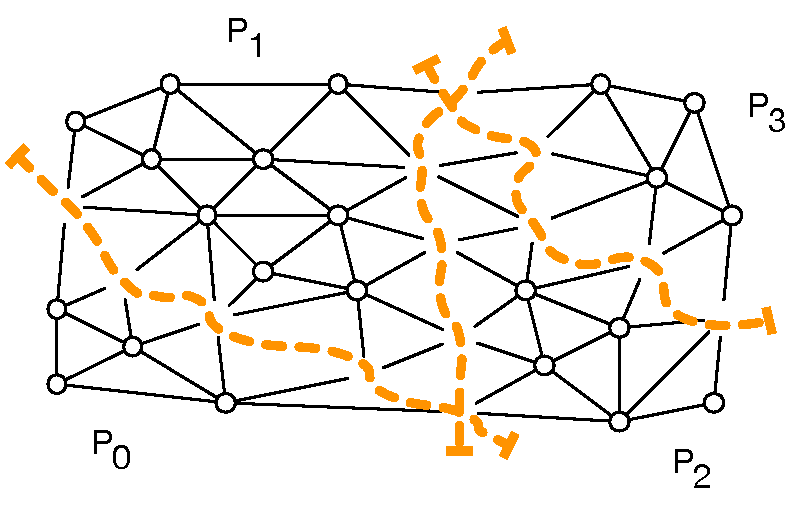
\includegraphics[scale=0.6]{sparsetiling/figures/partiotioned.pdf}
\caption{Partitioning of the seed loop. The vertices are illustrated to make the connectivity of the mesh clear, although they do not belong to any partition yet.}
\label{fig:st-initial-part-sm}
\end{figure}

As detailed in the next two sections, the inspection proceeds by populating $T_i$ with iterations from $L_1$ and $L_2$. The challenge of this task is guaranteeing that all data dependencies -- read after write, write after read, write after write -- are honored. The output of the inspector is eventually passed to the executor. The inspection carries sufficient information for computing sets of tiles in parallel. $T_i$ is always executed by a single thread/process and the execution is atomic; that is, it does not require communication with other threads/processes. When executing $T_i$, first all iterations from $L_0$ are executed, then all iterations from $L_1$ and finally those from $L_2$.

\subsection*{Inspection for Shared-Memory Parallelism}
Similarly to OP2, to achieve shared-memory parallelism we use coloring. Two tiles that are given the same color can be executed in parallel by different threads. Two tiles can have the same color if they are not connected, because this ensures the absence of race conditions through indirect memory accesses during parallel execution. In the example we can use three colors: red (R), green (G), and blue (B). $T_0$ and $T_3$ are not connected, so they are assigned the same color. The colored tiles are shown in Figure~\ref{fig:st-loop-0}. In the following, with the notation $T_i^c$ we indicate that the $i$-th tile has color $c$. 

\begin{figure}
\centering
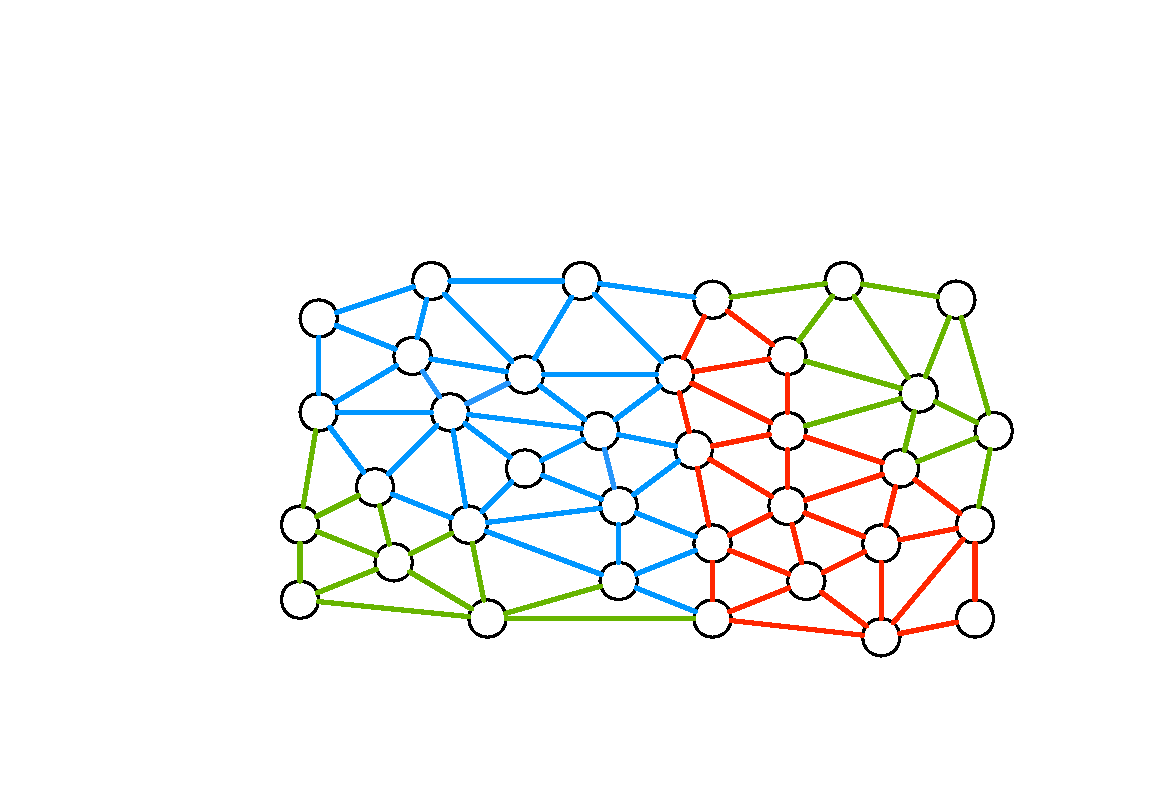
\includegraphics[scale=0.6]{sparsetiling/figures/loop_0.pdf}
\caption{A snapshot of the mesh after tiling $L_0$.}
\label{fig:st-loop-0}
\end{figure}

To populate $[T_0^G,\ T_1^B,\ T_2^R,\ T_3^G]$ with iterations from $L_1$ and $L_2$, we first have to establish a total ordering for the execution of partitions with different colors. Here, we assume the following order: green (G), blue (B), and red (R). This implies, for instance, that \textit{all iterations} assigned to $T_1^B$ must be executed \textit{before all iterations} assigned to $T_2^R$. By ``all iterations'' we mean the iterations from $L_0$ (determined by the seed partitioning) as well as the iterations that will later be assigned from tiling $L_1$ and $L_2$. We assign integer positive numbers to colors to reflect their ordering, where a smaller number means higher execution priority. We can assign, for example, 0 to green, 1 to blue, and 2 to red.

To schedule the iterations of $L_1$ to $[T_0^G,\ T_1^B,\ T_2^R,\ T_3^G]$, we need to compute a \textit{projection} for any write or local reduction performed by $L_0$. The projection required by $L_0$ is a function $\phi : V \rightarrow \mathbb{T}$ mapping the vertices in $V$ -- as indirectly incremented during the execution of $L_0$, see Listing~\ref{code:tiling-runningexample} -- to a tile $T_i^c \in \mathbb{T}$. Consider the vertex $v_0$ in Figure~\ref{fig:st-loop-0-proj}. $v_0$ has 7 incident edges, 2 of which belong to $T_0^G$, while the remaining 5 to $T_1^B$. Since we established that $G \prec B$, $v_0$ can only be read after $T_1^B$ has finished executing the iterations from $L_0$ (i.e., the 5 incident blue edges). We express this condition by setting $\phi(v_0) = T_1^B$. Observe that we can compute $\phi$ by iterating over $V$ and, for each vertex, applying the maximum function ($\operatorname{MAX}$) to the color of the adjacent edges. 

\begin{figure}
\centering
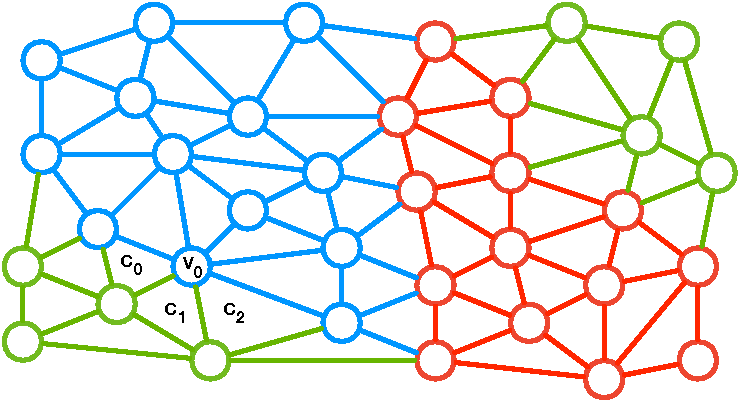
\includegraphics[scale=0.6]{sparsetiling/figures/loop_0_with_vertices.pdf}
\caption{The vertices are written by $L_0$, so a projection must be computed before tiling $L_1$. Here, the projection is represented by the colored vertices.}
\label{fig:st-loop-0-proj}
\end{figure}

\begin{figure}
\centering
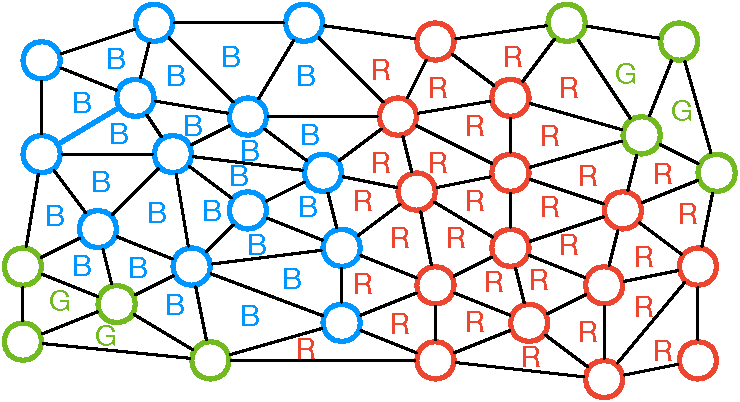
\includegraphics[scale=0.6]{sparsetiling/figures/loop_1.pdf}
\caption{A snapshot of the mesh after tiling $L_1$.}
\label{fig:st-loop-1}
\end{figure}

We now use $\phi$ to schedule $L_1$, a loop over cells, to the tiles. Consider again $v_0$ and the adjacent cells $[c_0,\ c_1,\ c_2]$ in Figure~\ref{fig:st-loop-0-proj}. These three cells have in common the fact that they are adjacent to both green and blue vertices. For $c_1$, and similarly for the other cells, we compute $\operatorname{MAX}(\phi(v_0),\ \phi(v_1),\ \phi(v_2)) = \operatorname{MAX}(B, G, G) = B = 1$. This establishes that $c_1$ must be assigned to $T_1^B$, because otherwise ($c_1$ assigned instead to $T_0^G$) a read to $v_0$ would occur before the last increment from $T_1^B$ took place. Indeed, we recall that the execution order, for correctness, must be ``all iterations from $[L_0, L_1, L_2]$ in the green tiles before all iterations from $[L_0, L_1, L_2]$ in the blue tiles''. The scheduling of $L_1$ to tiles is displayed in Figure~\ref{fig:st-loop-1}.

\begin{figure}[t]
\centering
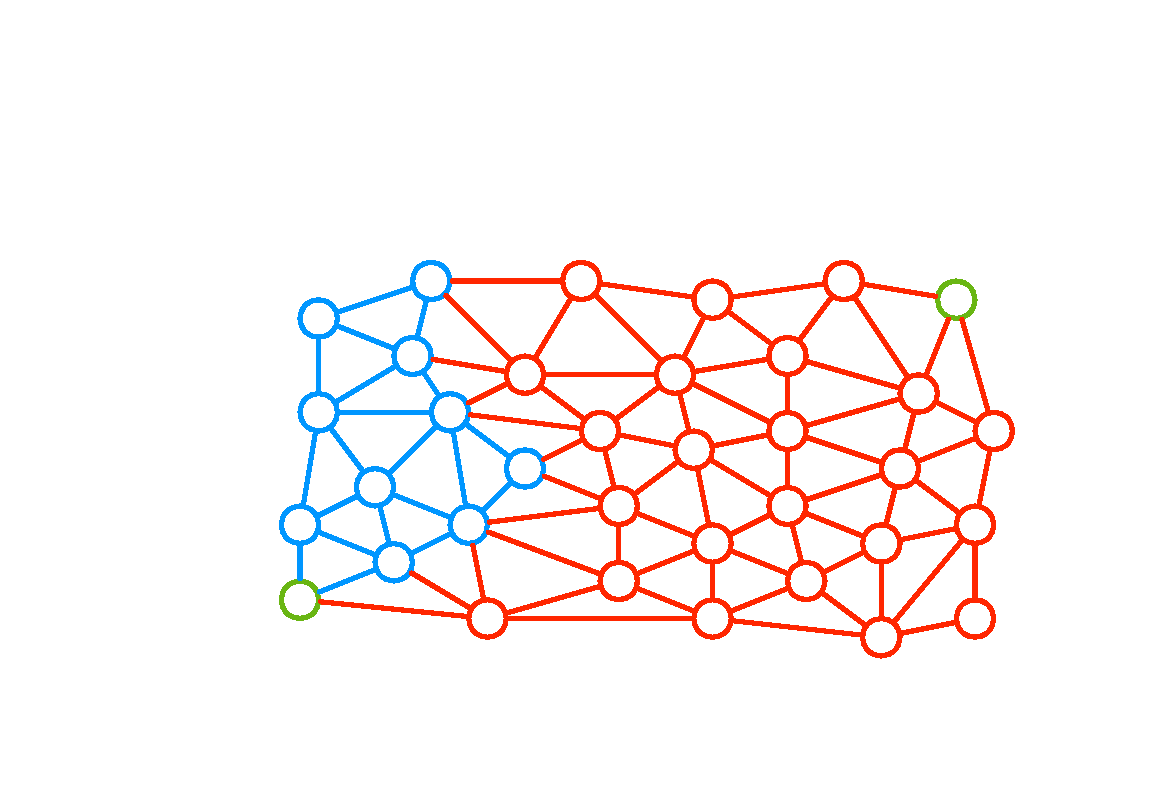
\includegraphics[scale=0.6]{sparsetiling/figures/loop_2.pdf}
\caption{A snapshot of the mesh after tiling $L_2$.}
\label{fig:st-loop-2}
\end{figure}

To schedule $L_2$ to $[T_0^G,\ T_1^B,\ T_2^R,\ T_3^G]$ we employ a similar process. Vertices are again written by $L_1$, so a new projection over $V$ will be necessary. Figure~\ref{fig:st-loop-2} shows the output of this last phase. 



\paragraph{Conflicting Colors}

\begin{figure}[hbtp]
\centering
\begin{subfigure}[b]{0.33\textwidth}
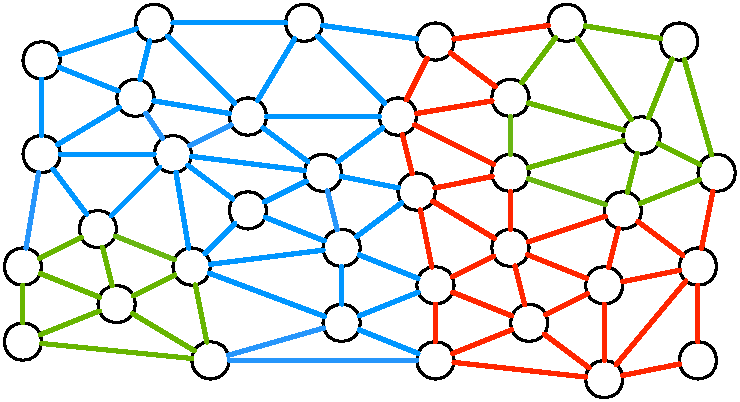
\includegraphics[width=\textwidth]{sparsetiling/figures/loop_0_conflicts.pdf}
\caption{After tiling $L_0$}
\label{fig:st-conflicts-a}
\end{subfigure}%
~ 
\begin{subfigure}[b]{0.33\textwidth}
\centering
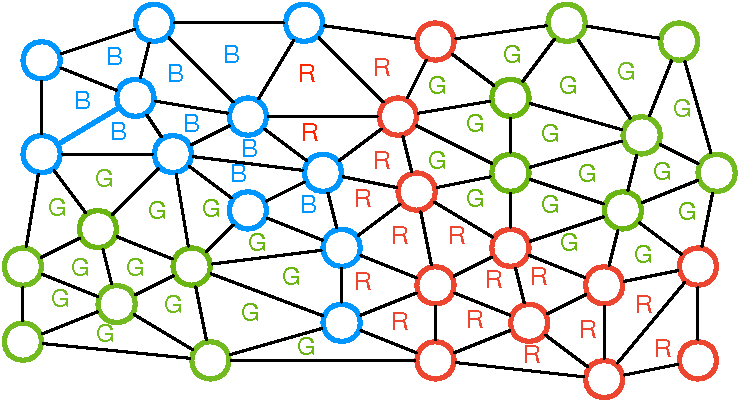
\includegraphics[width=\textwidth]{sparsetiling/figures/loop_1_conflicts.pdf}
\caption{After tiling $L_1$}
\label{fig:st-conflicts-b}
\end{subfigure}%
~
\begin{subfigure}[b]{0.34\textwidth}
\centering
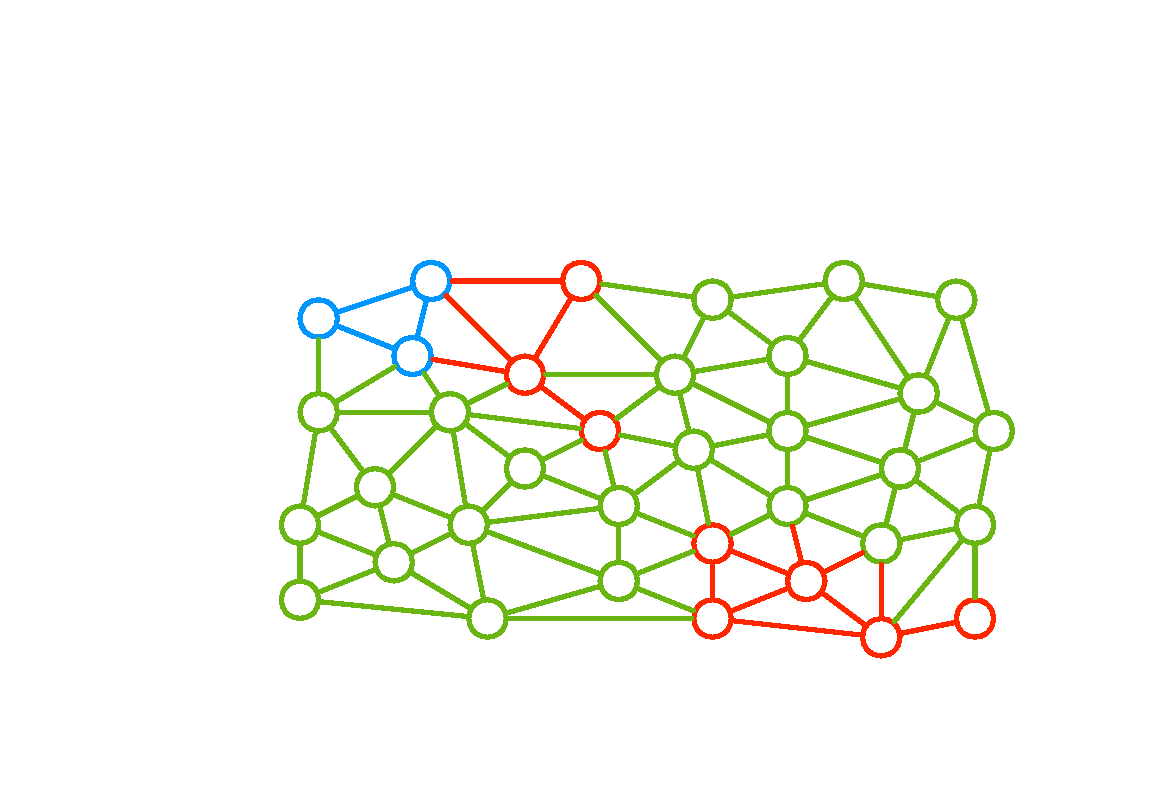
\includegraphics[width=\textwidth]{sparsetiling/figures/loop_2_conflicts.pdf}
\caption{After tiling $L_2$}
\label{fig:st-conflicts-c}
\end{subfigure}%

\caption{Tiling the program in Listing~\ref{code:tiling-runningexample} for shared-memory parallelism can lead to conflicts. Here, the two green tiles eventually become adjacent, creating race conditions.}
\label{fig:st-conflicts}
\end{figure}

It is worth noting how $T_2^R$ ``consumed'' the frontier elements of all other tiles every time a new loop was scheduled. Tiling a loop chain consisting of $k$ loops has the effect of expanding the frontier of a tile of at most $k$ vertices. With this in mind, we re-inspect the loop chain of the running example, although this time employing a different execution order -- blue (B), red (R), and green (G) -- and a different seed partitioning. Figure~\ref{fig:st-conflicts} shows that, by applying the same procedure described in this section, $T_0^G$ and $T_3^G$ will eventually become adjacent. This violates the precondition that {\it tiles can be given the same color, and thus run in parallel, as long as they are not adjacent}. Race conditions during the execution of iterations belonging to $L_2$ are now possible. This problem will be solved in Section~\ref{sec:tiling:inspector}.


\subsection*{Inspection for Distributed-Memory Parallelism}

In the case of distributed-memory parallelism, the mesh is partitioned and distributed to a set of processes. As shown in Listing~\ref{code:tiling-struct}, neighboring processes may exchange (MPI) messages before executing a loop $L_j$. A message includes all ``dirty'' dataset values required by $L_j$ modified by any $L_k$, with $L_k \prec L_j$. In the running example, $L_0$ writes to vertices, so a subset of values associated with border vertices must be communicated prior to the execution of $L_1$. To apply sparse tiling, the idea is to push all communications at the beginning of the loop chain: as we shall see, this increases the amount of data to be communicated, but also reduces  the number of synchronizations (only 1 synchronization between each pair of neighboring processes per loop chain execution).

From Section~\ref{sec:tiling:lc-unstruct} it is known that, in a loop chain, a set is logically split into three regions, \textit{core}, \textit{boundary}, and \textit{non-exec}. The boundary tiles, which originate from the seed partitioning of the boundary region, will include all iterations that cannot be executed until the communications have terminated. The procedure described for shared-memory parallelism -- now performed individually by each process on a partition of the input mesh -- is modified as follows:
\begin{enumerate}
\item The core region of the seed loop $L_0$ is partitioned into tiles. Unless aiming for a mixed distributed/shared-memory scheme, there is no need to assign identical colors to unconnected tiles, as a process will execute its own tiles sequentially. Colors are assigned increasingly, with $T_i$ given color $i$. As long as tiles with contiguous ID are also physically contiguous in the mesh, this assignment retains spatial locality when ``jumping'' from executing $T_i$ to $T_{i+1}$.
\item The same process is applied to the boundary region. Thus, a situation in which a tile includes iterations from both the core and the boundary regions is prevented by construction. Further, all tiles within the boundary region are assigned colors higher than those used for the core tiles. This constrains the execution order: no boundary tiles will be executed until all core tiles are computed.
\item We map the whole non-exec region of $L_0$ to a single special tile, $T_{ne}$. This tile has the highest color and will actually never be executed. 
\end{enumerate}

\begin{figure}[b]
\centering
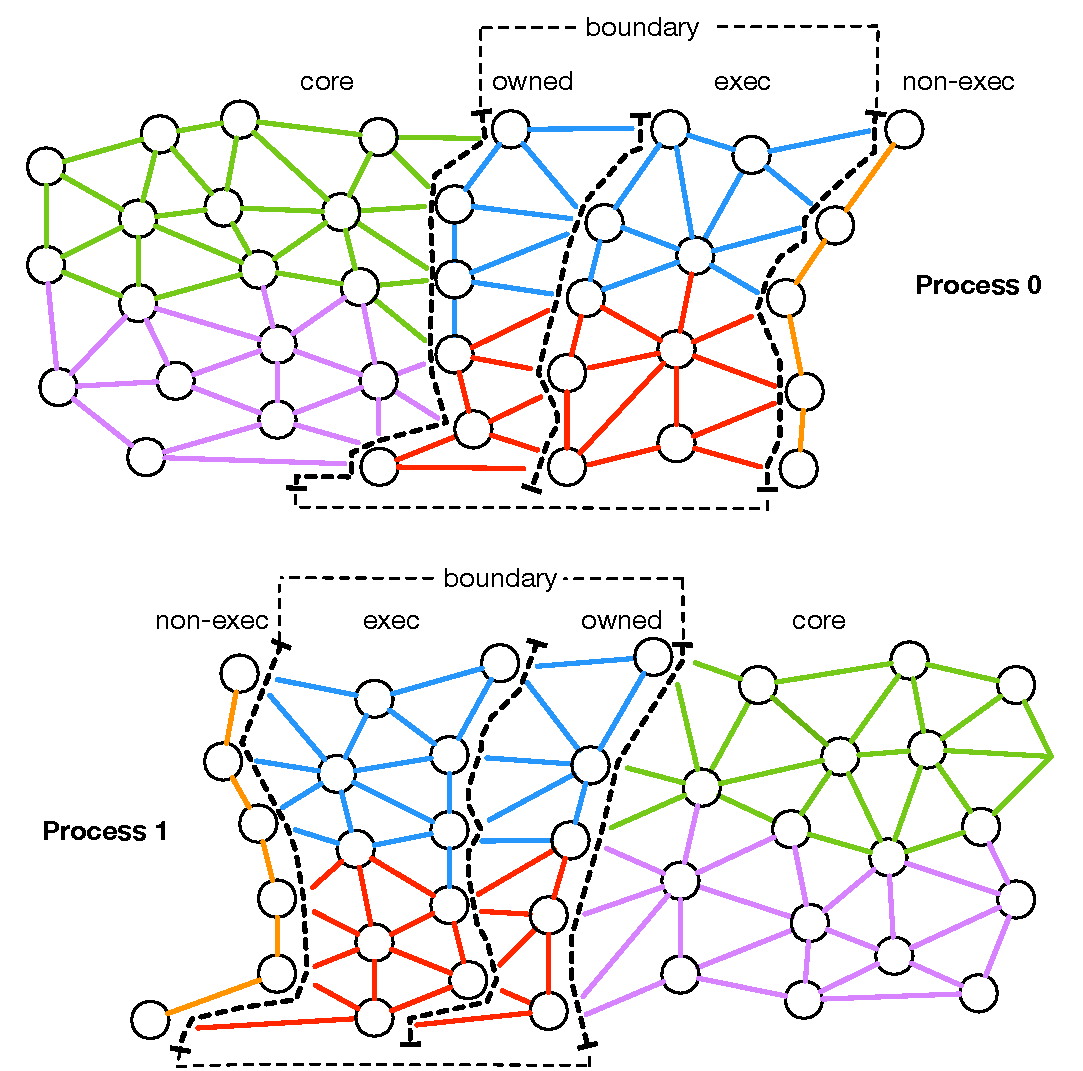
\includegraphics[scale=0.6]{sparsetiling/figures/mpi_loop0.pdf}
\caption{A snapshot of the two mesh partitions on {\tt Process 0} and {\tt Process 1} after inspecting the seed loop $L_0$ for distributed-memory parallelism. On each process, there are five tiles in total: two in the core region (green and violet), two in the boundary region (red and light blue), and $T_{ne}$. The boundary tiles can safely cross the owned and exec sub-regions (i.e., the private local iterations and the iterations to be redundantly computed, respectively). However, no tile can include iterations from both the core and the boundary regions. }
\label{fig:st-mpi-init}
\end{figure}

\begin{figure}[t]
\centering
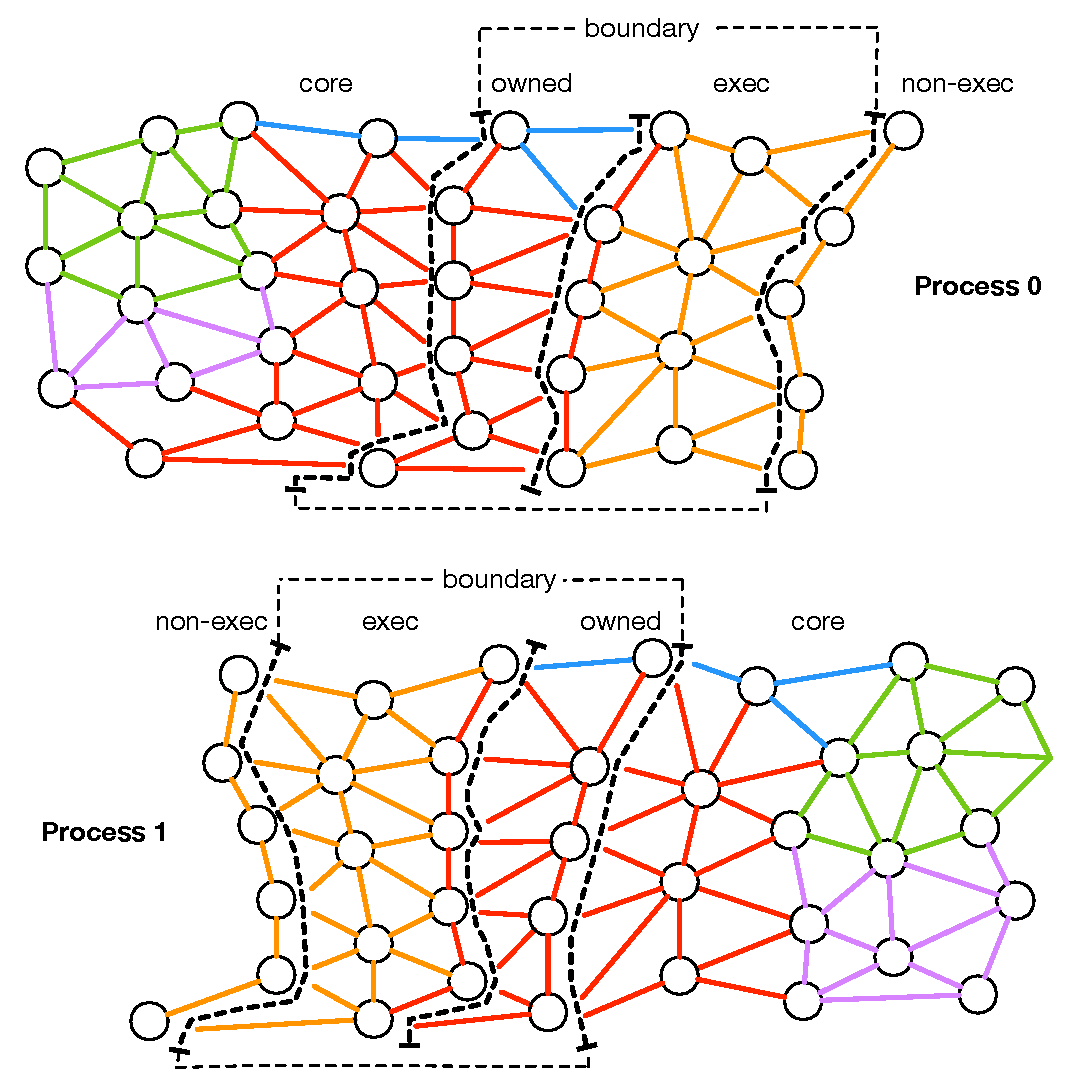
\includegraphics[scale=0.6]{sparsetiling/figures/mpi_loop2.pdf}
\caption{A snapshot of the two mesh partitions on {\tt Process 0} and {\tt Process 1} at the end of the inspection for distributed-memory parallelism. $T_{ne}$ expands over the boundary region, which minimizes the amount of redundant computation to be performed. At the end of the execution phase, the orange edges will contain ``dirty  values'', but correctness is not affected as the exec region only includes off-process data. The boundary tiles expand over the core region: this is essential for correctness since none of the red and blue entities from $[L_0,\ L_1,\ L_2]$ can be executed until the MPI communications have terminated.}
\label{fig:st-mpi-growth}
\end{figure}

From this point on, the inspection proceeds as in the case of shared-memory parallelism. The application of the $\operatorname{MAX}$ function when scheduling $L_1$ and $L_2$ makes higher color tiles (i.e., those having lower priority) ``expand over'' lower color ones. 

In Figure~\ref{fig:st-mpi-init}, a mesh is partitioned over two processes and a possible seed partitioning and tiling of $L_0$ illustrated. We observe that the two boundary tiles (the red and light blue ones) will expand over the core tiles as $L_1$ and $L_2$ are tiled, which eventually results in the scheduling illustrated in Figure~\ref{fig:st-mpi-growth}. Roughly speaking, if a loop chain consists of $n$ loops and, on each process, $n-1$ extra layers of iterations are provided (the exec regions in Figure~\ref{fig:st-mpi-init}), then all boundary tiles are correctly computed. 

The schedule produced by the inspector is subsequently used by the executor. On each process, the executor starts with triggering the MPI communications required for the computation of boundary tiles. All core tiles are then computed, since no data from the boundary region is necessary. Hence, computation is overlapped with communication. As all core tiles are computed and the MPI communications terminated, the boundary tiles can finally be computed.

\paragraph{Efficiency considerations}
The underlying hypothesis is that the increase in data locality will outweigh the overhead induced by the redundant computation and by the bigger volume of data exchanged. This is motivated by several facts: (i) the loops being memory-bound;  (ii) the core region being much larger than the boundary region; (iii) the amount of redundant computation being minimized through the special tile $T_{ne}$, which progressively expands over the boundary region, thus avoiding unnecessary calculations.


\section{Data Dependency Analysis for Loop Chains}

As with all loop optimizations that reschedule the iterations in a sequence of loops, any sparse tiling must satisfy the data dependencies. The loop chain abstraction, which we have described in Section~\ref{sec:tiling:lc}, provides enough information to construct an inspector which analyzes all of the dependencies in a computation and builds a legal sparse tiling. We recall that one of the main assumptions in a loop chain is that each loop is fully parallel or, equivalently, that there are no loop carried dependencies.

The descriptors in the loop chain abstraction enable a general derivation of the storage-related dependencies between loops in a loop chain. The storage related dependencies between loops can be described as either flow (read after write), anti (write after read), or output (write after write) dependencies. In the following, assume that loop $L_x$, having iteration space $S_x$, always comes before loop $L_y$, having iteration space $S_y$, in the loop chain. Let us identify a descriptor of a loop $L$ with $m_{S_i \rightarrow S_j}^{\mathrm{mode}}$: this simply indicates that the loop $L_i$ has iteration space $S_i$ and uses a map $m$ to write/read/increment elements (respectively, $\texttt{mode} \in \lbrace w, r, i\rbrace$) in the space $S_j$.

The flow dependencies can then be enumerated by considering pairs of points ($\vec{i}$ and $\vec{j}$) in the iteration spaces of the two loops $L_x$ and $L_y$:
\[
	\{ \vec{i} \rightarrow \vec{j} \; | \; \vec{i} \in S_x \wedge \vec{j} \in S_y \wedge 
	m_{S_x\rightarrow S_z}^{w}(\vec{i}) \cap m_{S_y \rightarrow S_z}^{r}(\vec{j}) \ne \emptyset \}.
\]
Anti and output dependencies are defined in a similar way. The anti dependencies for all pairs of loops $L_x$ and $L_y$ are:
\[
	\{ \vec{i} \rightarrow \vec{j} \; | \; \vec{i} \in S_x \wedge \vec{j} \in S_y \wedge 
	m_{S_x\rightarrow S_z}^{r}(\vec{i}) \cap m_{S_y \rightarrow S_z}^{w}(\vec{j}) \ne \emptyset \}.
\]
While the output dependencies between loops $L_x$ and $L_y$ are:
\[
	\{ \vec{i} \rightarrow \vec{j} \; | \; \vec{i} \in S_x \wedge \vec{j} \in S_y \wedge 
	m_{S_x\rightarrow S_z}^{w}(\vec{i}) \cap m_{S_y \rightarrow S_z}^{w}(\vec{j}) \ne \emptyset \}.
\]
In essence, there is a storage-related data dependence between two iterations from different loops (and therefore between the tiles they are placed in) when one of those iterations writes to a data element and the other iteration reads from or writes to the same data element.

There are local reductions, or ``reduction dependencies'' between two or more iterations of the same loop when those iterations ``increment'' the same location(s); that is, when they read, modify with a commutative and associative operator, and write to the same location(s). The reduction dependencies in $L_x$ are:
\[
	\{ \vec{i} \rightarrow \vec{j} \; | \; \vec{i} \in S_x \wedge \vec{j} \in S_x \wedge m_{S_x\rightarrow S_z}^{i}(\vec{i}) \cap m_{S_x \rightarrow S_z}^{i}(\vec{j}) \ne \emptyset \}.
\]
The reduction dependencies between two iterations within the same loop indicates that those two iterations must be executed atomically with respect to each other.

As seen in the example in Section~\ref{sec:tiling:examples}, our inspector algorithm handles data dependencies, including those between non-adjacent loops, by tracking \textit{projections}. In the next section we explain how projections are constructed and used.

%In order to schedule $L$ to tiles, an up-to-date projection for each set $S$ accessed by $L$ must be available. For example, assume that $S$ is read by $L_k$ and is written by both $L_i$ and $L_j$. In the loop chain, the loops are in the order $L_i \prec ... \prec L_j \prec ... \prec L_k$. Let us denote by $\phi_S$ the projection for $S$. Each time that a loop accessing $S$ in write mode is inspected for scheduling, $\phi_S$ must be updated. When eventually scheduling $L_k$, therefore, an up-to-date snapshot of $\phi_S$ (i.e., the one produced right after tiling $L_j$) will be used to compute a legal tiling.

\clearpage


\section{Formalization}
\label{sec:tiling:algo}

\subsection{The Generalized Sparse Tiling Inspector}
\label{sec:tiling:inspector}

The pseudo-code for the generalized sparse tiling inspector is shown in Algorithm~\ref{algo:st-inspector}. Given a loop chain and a ``seed'' tile size, the algorithm produces a schedule suitable for mixed distributed/shared-memory parallelism. In the following, we elaborate on the main steps of the algorithm. The notation used throughout the section is summarized in Table~\ref{table:st-summary-notation}.

\begin{table}[h]
\centering
\begin{tabulary}{1.0\columnwidth}{C|C}
\hline
Symbol & Meaning \\
\hlineB{4}
$\mathbb{L}$ & The loop chain \\
$L_j$ & The $j$-th loop in $\mathbb{L}$ \\ 
$S_j$ & The iteration space of $L_j$ \\
$S_j^{c}$, $S_j^{b}$, $S_j^{ne}$ & The core, boundary, and non-exec regions of $S_j$ \\ 
$S$ & A generic set in $\mathbb{L}$ \\
$D$ & A descriptor of a loop \\
$r$, $w$, $i$ & Possible values for $D$.mode \\
$\mathbb{T}$ & The set of all tiles \\
$\mathbb{T}[i]$ & Accessing the $i$-th tile \\
%$T_i^{c}$, $T_i^{b}$ & the $i$-th tile over the core and boundary regions \\
$\phi_S$ & A projection $\phi_S : S \rightarrow \mathbb{T}$ \\
$\Phi$ & The set of all available projections \\
$\sigma_j$ & A tiling function $\sigma_j : S_j \rightarrow \mathbb{T}$ for $L_j$ \\
$ts$ & seed tile size \\
\hline
\end{tabulary}
\caption{Summary of the notation used throughout the section.}
\label{table:st-summary-notation}
\end{table}



\setcounter{algocf}{0}% Modify counter of algorithm
\begin{algorithm}[!t]

\SetKwData{SeedMap}{seed$\_$map}
\SetKwData{Conflicts}{conflicts}
\SetKwData{C}{C}
\SetKwFunction{AFC}{add$\_$fake$\_$connection}
\SetKwFunction{IFC}{has$\_$conflicts}
\SetKwFunction{CLM}{compute$\_$local$\_$maps}
\SetKwFunction{Color}{color}
\SetKwFunction{Partition}{partition}
\SetKwFunction{FindMap}{find$\_$map}
\SetKwFunction{Project}{project}
\SetKwFunction{Assign}{assign}
\SetKwFunction{Tile}{tile}

\kwInput{The loop chain $\mathbb{L} = [L_0,\ L_1,\ ...,\ L_{n-1}]$, a tile size $ts$}
\kwOutput{A set of tiles $\mathbb{T}$, populated with iterations from $\mathbb{L}$}
\nonl ~\\
\Comment{Initialization}
$seed \gets 0$\;
$\Phi \gets \emptyset$\;
$\C \gets \perp$\;
\nonl ~\\
\Comment{Creation of tiles}
$\sigma_{seed}$, $\mathbb{T} \gets$ \Partition{$S_{seed}$, $ts$}\;
\SeedMap $\gets$ \FindMap{$S_{seed}$, $\mathbb{L}$}\;
\Conflicts $\gets$ \False\;
\nonl ~\\
\Comment{Schedule loops to tiles}
\Do{\Conflicts}{
  \Color{$\mathbb{T}$, \SeedMap}\;
   \nonl ~\\
  \For{$j=1$ \KwTo $n-1$}{ \label{algo:st-tiling-loop}
    \Project{$L_{j-1}$, $\sigma_{j-1}$, $\Phi$, $C$}\;
    $\sigma_j \gets$ \Tile{$L_j$, $\Phi$}\;
    \Assign{$\sigma_j$, $\mathbb{T}$}\;
  }
  \nonl ~\\
  \If{\IFC{\C}}{
    \Conflicts $\gets$ \True\;
    \AFC{\SeedMap, \C}\;
  }
}
\nonl ~\\
\Comment{Inspection successful, create local maps and return}
\CLM{$\mathbb{T}$}\;
\Return{$\mathbb{T}$}
\caption{The inspection algorithm}
\label{algo:st-inspector}
\end{algorithm}





\paragraph{Choice of the seed loop}
The seed loop $L_{seed}$ is used to initialize the tiles. Theoretically, any loop in the chain can be chosen as seed. Supporting distributed-memory parallelism, however, is cumbersome if $L_{seed} \neq L_0$. This is because more general schemes for partitioning and coloring would be needed to ensure that no iterations in any $S_j^{b}$ are assigned to a core tile. A limitation of our inspector algorithm in the case of distributed-memory parallelism is that it must be $L_{seed} = L_0$. 

In the special case in which there is no need to distinguish between core and boundary tiles (because a program is executed on a single shared-memory system), $L_{seed}$ can be chosen arbitrarily. If we however pick $L_{seed}$ in the middle of the loop chain ($L_0 \prec ... \prec L_{seed} \prec ...$), a mechanism for constructing tiles in the reverse direction (``backwards''), from $L_{seed}$ towards $L_0$, is necessary. In~\cite{st-paper}, we propose two ``symmetric'' algorithms to solve this problem, \textit{forward tiling} and \textit{backward tiling}, with the latter using the $\operatorname{MIN}$ function in place of $\operatorname{MAX}$ when computing projections. For ease of exposition, and since in the fundamental case of distributed-memory parallelism we are imposing $L_{seed} = L_0$, we here neglect this distinction\footnote{The algorithm implemented in the library presented in Section~\ref{sec:tiling:impl-slope} supports backwards tiling for shared-memory parallelism.}. 

%\textit{Note: in real applications loops over ``subsets'' are possible; for instance, a loop over the exterior facets of the mesh. If one such loop is picked as seed, then the inspection is aborted.}



\paragraph{Tile initialization}

\begin{table}[ht]
\centering
\begin{tabulary}{1.0\columnwidth}{P{2.7cm} | P{8.5cm}}
\hline
Field & Possible values \\
\hlineB{4}
{\em region} & core, boundary, non-exec \\
{\em iterations lists} & one list of iterations $[T_i]_j$ for each $L_j \in \mathbb{L}$\\ 
{\em local maps} & one list of local maps for each $L_j \in \mathbb{L}$; one local map for each map used in $L_j$\\
{\em color} & an integer representing the execution priority \\ 
\hline
\end{tabulary}
\caption{The tile data structure.}
\label{table:st-tile-structure}
\end{table}

Let $ts$ be the user-specified average tile size. The algorithm starts with partitioning $S_{seed}^{c}$ into $m$ subsets $\lbrace P_0, P_1, ..., P_{m-1}\rbrace$ such that $|P_i| = ts$ (except possibly for $P_{m-1}$), $P_i \cap P_j = \emptyset$, and $\cup_{i = 0}^{m-1} P_i = S_{seed}^{c}$. Among all possible legal partitionings, we choose the one that splits $S_{seed}^c$ into blocks of $ts$ contiguous iterations, with $P_0 = \lbrace 0, ..., ts-1\rbrace$, $P_1 = \lbrace ts, ..., 2 ts - 1\rbrace$, and so on. We analogously partition $S_{seed}^{b}$ into $k$ subsets. We create $m+k+1$ tiles, one for each of these partitions and one extra tile for $S_{seed}^{ne}$. We therefore have $\mathbb{T} = \lbrace T_0^c, ..., T_{m-1}^c, T_m^{b}, ..., T_{m+k-1}^b, T_{m+k}^{ne} \rbrace$. 

A tile $T_i$ has four fields, as summarized in Table~\ref{table:st-tile-structure}. 

\begin{itemize}
\item The {\em region} is used by the executor to schedule tiles in a given order. This field is set right after the partitioning of $L_{seed}$, as a tile (by construction) exclusively belongs to $S_{seed}^c$, $S_{seed}^b$, or $S_{seed}^{ne}$.
\item The {\em iterations lists} contain the iterations in $\mathbb{L}$ that $T_i$ will have to execute. There is one {\em iterations list} $[T_i]_j$ for each $L_j \in \mathbb{L}$. At this stage of the inspection we have $[T_i]_{seed} = [T_i]_0 = P_i$, whereas still $[T_i]_j = \emptyset$ for $j=1,...,n$.
\item {\em Local maps} may be used for performance optimization by the executor in place of the global maps provided through the loop chain; this will be discussed in more detail in Section~\ref{sec:tiling:seigen}.
\item The {\em color} gives a tile a scheduling priority. If shared-memory parallelism is requested, adjacent tiles are given different colors (the adjacency relation is determined through the maps available in $\mathbb{L}$). Otherwise, colors are assigned in increasing order (i.e., $T_i$ is given color $i$). The boundary tiles are always given colors higher than that of core tiles; the non-exec tile has the highest color. The assignment of colors is carried by the function {\tt color} in Listing~\ref{algo:st-inspector}.
\end{itemize}



\paragraph{Populating tiles by tracking data dependencies}
To schedule a loop to tiles we use projections. A projection is a function $\phi_S : S \rightarrow \mathbb{T}$. Initially, the projections set $\Phi$ is empty. Each time a loop is tiled, $\Phi$ may be added some new projections or old projections may be updated. $\Phi$, and consequently the tiling functions for all loops in $\mathbb{L}$, are derived incrementally (within the loop at line~\ref{algo:st-tiling-loop} in Listing~\ref{algo:st-inspector}) starting from $\sigma_{seed} : S_{seed} \rightarrow \mathbb{T}$, the tiling function of $L_{seed}$. In the following, we discuss in detail how projections and tiling functions are constructed. 


\paragraph{Deriving a projection from a tiling function}

\begin{algorithm}[htp]
\SetKwData{Descriptors}{descriptors}
\SetKwData{Arity}{arity}
\SetKwData{AT}{$T_{last}$}
\SetKwData{MC}{max$\_$color}
\SetKwData{IM}{inverse$\_$map}
\SetKwData{Size}{size}
\SetKwData{Map}{map}
\SetKwData{Mode}{mode}
\SetKwData{D}{D}
\SetKwData{C}{C}
\SetKwData{Values}{values}
\SetKwData{Offset}{offset}
\SetKwData{Color}{color}
\SetKwFunction{MapInvert}{map$\_$invert}
\SetKwFunction{Update}{update}

\kwInput{A loop $L_j$, a tiling function $\sigma_j$, the projections set $\Phi$, the conflicts matrix $C$}
\KwResult{Update $\Phi$ and $C$}
\nonl ~\\
\ForEach{\D $\in$ $L_j$.\Descriptors}{
  \eIf{\D .\Map $==$ $\perp$}{
    $\Phi = \Phi \cup \sigma_{i}$\;
  }{
    \IM $\gets$ \MapInvert{\D .\Map}\;
    $S_t$, $S_j$, \Values, \Offset $\gets$ \IM\;
    $\phi_{S_t} \gets \perp$\; 
    \For{$e=0$ \KwTo $S_t$.\Size}{ \label{algo:st-projection-parallel}
      \For{$k= \Offset[e]$ \KwTo $\Offset[e+1]$}{
        \AT = $\mathbb{T}[\Values[k]]$\;
        \MC $\gets$ MAX($\phi_{S_{t}}[e]$.\Color, \AT .\Color)\;
        \If{\MC $\neq$ $\phi_{S_{t}}[e]$.\Color}{
          $\phi_{S_{t}}[e] \gets$ \AT\;
        }
      }
    }
    \Update{\C, $\mathbb{T}$, $\phi_{S_{t}}$}\;
    $\Phi = \Phi \cup \phi_{S_{t}}$\;
  }
}
\caption{Projection of a tiled loop}
\label{algo:st-projection}
\end{algorithm}

Algorithm~\ref{algo:st-projection} takes as input (the descriptors of) $L_{j}$ and its tiling function $\sigma_{j} :S_j \rightarrow \mathbb{T}$ to update $\Phi$. The algorithm also updates the conflicts matrix $C \in \mathbb{N}^{m \times m}$, which indicates whether two tiles having the same color will become adjacent once $L_{j+1}$ is tiled. 

A projection tells what tile a set element logically belongs to at a given point of the inspection. A new projection $\phi_{S}$ is needed if the elements of $S$ are written by a loop. Let us consider the non-trivial case in which writes or increments occur indirectly through a map $M : S_j \rightarrow S_t^0 \times S_t^1 \times ... \times S_t^{a-1}$. To compute $\phi_{S_{t}}$, we first determine the inverse map (an example is shown in Figure~\ref{fig:st-inverse-map}). Then, we iterate over all elements of $S_t$ and, for each $e \in S_t$, we determine the last tile that writes to $e$, say $T_{last}$. This is accomplished by applying the $\operatorname{MAX}$ function over the color of the tiles accessing $e$. We finally simply set $\phi_{S_{t}}[e] = T_{last}$. 


\begin{figure}[h]
\begin{CenteredBox}
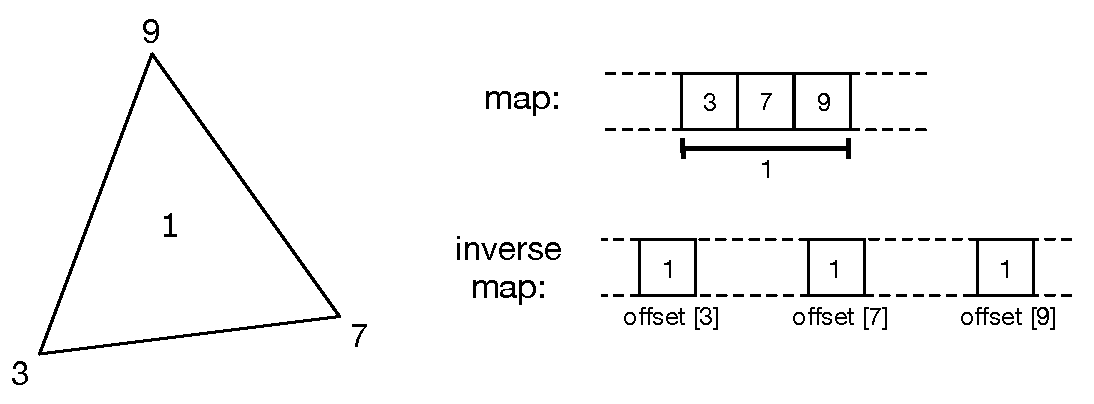
\includegraphics[scale=0.7]{sparsetiling/figures/inverse_map}
\end{CenteredBox}
\caption{Representation of an inverse map. The original map shows that the triangular cell $1$ is adjacent to three vertices, namely $3$, $7$, and $9$. The inverse map associates vertices to cells. Since the mesh is unstructured, different vertices can be incident to a different number of cells. The array {\tt offset} determines the distance between two consecutive vertices in the inverse map. For instance, all entries in the inverse map between {\tt offset[3]} and {\tt offset[4]} are cells incident to vertex $3$ (in the illustrated case, the first of these is cell $1$).}
\label{fig:st-inverse-map}
\end{figure}

% ($C[i,j] = 1$ implies that $T_i$ and $T_j$ have the same color and will become adjacent after tiling $L_{i-1}$).

\paragraph{Deriving a tiling function from the available projections}

\begin{algorithm}[htp]
\SetKwData{Descriptors}{descriptors}
\SetKwData{Arity}{arity}
\SetKwData{AT}{adjacent$\_$tile}
\SetKwData{MC}{max$\_$color}
\SetKwData{Size}{size}
\SetKwData{Map}{map}
\SetKwData{D}{D}
\SetKwData{Values}{values}
\SetKwData{Color}{color}

\kwInput{A loop $L_{j}$, the projections set $\Phi$}
\kwOutput{The tiling function $\sigma_{j}$}
\nonl ~\\
$\sigma_j \gets \perp$\;
\ForEach{\D $\in$ $L_j$.\Descriptors}{
  \eIf{\D .\Map $==$ $\perp$}{
    $\sigma_j \gets \Phi[S_j]$\;    
  }{
    \Arity $\gets$ D.\Map .\Arity\;
    $\phi_{S} \gets \Phi[\D.\Map.S_{j}]$\;
    \For{$e=0$ \KwTo $S_j$.\Size}{ \label{algo:st-tiling-parallel}
       $\sigma_j[e] \gets T_{\perp}$ \;
      \For{$k=0$ \KwTo \Arity}{
        \AT $\gets \phi_{S}[\D.\Map .\Values[e*\Arity + k]]$\;
        \MC $\gets$ MAX($\sigma_j[e]$.\Color, \AT .\Color)\;
        \If{\MC $\neq$ $\sigma_j[e]$.\Color}{
          $\sigma_j[e] \gets$ \AT\;
        }
      }
    }
  }
}
\Return{$\sigma_j$}
\caption{Building a tiling function}
\label{algo:st-tiling}
\end{algorithm}

Using $\Phi$, we compute $\sigma_j$ as described in Algorithm~\ref{algo:st-tiling}. The algorithm is similar to the projection of a tiled loop, with the main difference being that now we use $\Phi$ to schedule iterations correctly. Finally, $\sigma_j$ is inverted and the iterations are added to the corresponding iteration lists $[T_i]_j$, for all $T_i \in \mathbb{T}$. 


\paragraph{Detection of conflicts}
If $C$ indicates the presence of at least one conflict, say between $T_{i_1}$ and $T_{i_2}$, we add a ``fake connection'' between these two tiles and loop back to the coloring stage. $T_{i_1}$ and $T_{i_2}$ are now connected, so they will be assigned different colors. 
%Otherwise, a legal tiling has now been computed. 


\paragraph{History of the algorithm}
A first algorithm for sparse tiling inspection was developed by the author of this thesis in conjunction with researchers from multiple institutions, and was introduced in~\cite{st-paper}. In this section, a new, enhanced version of that algorithm has been presented. In essence, the major differences are: (i) support for distributed-memory parallelism; (ii) use of mesh coloring instead of a task graph for tile scheduling; (iii) speculative inspection with backtracking if a coloring conflict is detected; (iv) use of sets, instead of datasets, for data dependency analysis; (v) use of inverse maps for parallelization of the projection and tiling routines; (vi) computation of local maps. Most of these changes contributed to reduce the inspection cost.

\subsection{The Generalized Sparse Tiling Executor}

\begin{algorithm}[htpb]
\SetKwData{Color}{color}
\SetKwData{T}{T}
\SetKwFunction{SMC}{start$\_$MPI$\_$comm}
\SetKwFunction{EMC}{end$\_$MPI$\_$comm}
\SetKwFunction{GTBR}{group$\_$tiles$\_$by$\_$region}
\SetKwFunction{ET}{execute$\_$tile}

\kwInput{A set of tiles $\mathbb{T}$}
\KwResult{Execute the loop chain}
\nonl ~\\
$\mathbb{T}^{c}$, $\mathbb{T}^{b}$ $\gets$ \GTBR{$\mathbb{T}$}\;
\nonl ~\\
\SMC{}\;
\nonl ~\\
\ForEach{\Color}{
  \ForEach{$\T \in \mathbb{T}^{c}$ s.t. \T .\Color $==$ \Color}{ \label{algo:st-executor:parallel1}
    \ET{\T}\;
  }
}
\nonl ~\\
\EMC{}\;
\nonl ~\\
\ForEach{\Color}{
  \ForEach{$T \in \mathbb{T}^{b}$ s.t. \T .\Color $==$ \Color}{ \label{algo:st-executor:parallel2}
    \ET{\T}\;
  }
}
\caption{The executor algorithm}
\label{algo:st-executor}
\end{algorithm}


The sparse tiling executor is illustrated in Algorithm~\ref{algo:st-executor}. It consists of four main phases: (i) exchange of halo regions amongst neighboring processes through non-blocking communications; (ii) execution of core tiles (in overlap with communication); (iii) wait for the termination of the communications; (iv) execution of boundary tiles. 

As explained in Sections~\ref{sec:tiling:examples} and~\ref{sec:tiling:inspector}, a sufficiently deep halo region enables correct computation of the boundary tiles. Further, tiles are executed atomically, meaning that all iterations in a tile are computed without ever synchronizing with other processes. The depth of the boundary region, which affects the amount of off-process data to be redundantly computed, increases with the number $n$ of loops to be fused. In the example in Figure~\ref{fig:st-mpi-init}, there are $n=3$ loops, and three ``strips'' of extra vertices are necessary for correctly computing the fused loops without tile-to-tile synchronizations.

We recall from Section~\ref{sec:tiling:lc-unstruct} that the {\em depth} of the loop chain indicates the extent of the boundary region. This parameter imposes a limit to the number of fusible loops. If $\mathbb{L}$ includes more loops than the available boundary region -- that is, if $n > \text{{\em depth}}$ --  then $\mathbb{L}$ will have to be split into shorter loop chains, to be fused individually. As we shall see (Section~\ref{sec:tiling:impl-firedrake}), in our inspector/executor implementation the {\em depth} is controlled by the Firedrake's DMPlex module.

%For ease of explanation, this aspect has been neglected in the inspector algorithms described in the previous section. 

%Our inspector/executor strategy, therefore, works correctly as long as the loop chain has been ``dimensioned'' properly, with sufficient information in all $S^{b}$ regions 

%\paragraph{The execution of a tile}


\subsection{Computational Complexity of Inspection}


Let $N$ be the maximum size of a set in $\mathbb{L} = [L_0, L_1, ..., L_{n-1}]$ and let $M$ be the maximum number of sets accessed in a loop. If $a$ is the maximum arity of a map, then $K = a N$ is the maximum cost for iterating over a map. $K$ is also the worst-case cost for inverting a map. Let $p < 1$ be the probability that a conflict arises during inspection in the case of shared-memory parallelism; thus, the expected number of inspection rounds is $R = \frac{1}{1-p}$. Hence, the worst-case computational costs of the main inspection phases are as in Table~\ref{table:st-comp-cost}.

\begin{table}[h]
\centering
\begin{tabulary}{1.0\columnwidth}{P{2.7cm} | c | c}
\hline
Phase & Cost shared memory & Cost distributed memory \\
\hlineB{4}
Partitioning & $N$ & $N$ \\
Coloring & $R K $ & $N$ \\ 
Projection & $R (n M N K^2) $ & $n M N K^2 $ \\ 
Tiling & $R (n M N K) $ & $n M N K $ \\
Local maps & $n M$ & $n M$\\
\hline
\end{tabulary}
\caption{Worst-case computational costs of the main inspection phases.}
\label{table:st-comp-cost}
\end{table}

%LOCAL MAPS: Finally, for each $T_i \in \mathbb{T}$, for each $L_j \in \mathbb{L}$, for each map used in $L_j$, create a local map. 

\section{Implementation}
\label{sec:tiling:automation}
The implementation of automated generalized sparse tiling is distributed over three software modules. 
\begin{description}
\item[Firedrake] The framework for the automated solution of PDEs through the finite element method (Section~\ref{sec:bkg:fenics-and-firedrake}).
\item[PyOP2] Firedrake produces numerical kernels to be applied over sets of mesh components. The parallel iteration over the mesh is handled by PyOP2 (Section~\ref{sec:bkg:op2}).
\item[SLOPE] A library for writing generalized inspector/executor schemes, with primary focus on sparse tiling. PyOP2 uses SLOPE to apply sparse tiling to loop chains.
\end{description}

There are several reasons that motivate this structuring.
\begin{description}
\item[Simplicity of analysis] The abstractions used in Firedrake and PyOP2 drastically simplify the analysis of input programs. For example, from the parallel loop construct in PyOP2 (Section~\ref{sec:bkg:op2}) we can derive the information that we need to construct a loop chain.
\item[Flexibility] Inspector/executor schemes can be expressed at three different layers of abstraction: in Firedrake programs, in PyOP2 programs, or directly in C. It is extremely intuitive and simple to use sparse tiling in a Firedrake program. Once the regions of code to be sparse tiled are identified, the inspector/executor schemes are automatically derived in the PyOP2 implementation. In the case of a pure PyOP2 program, the generation of inspector/executor schemes is instead only partly automated, since the separation of a set into the core, boundary and non-exec regions for distributed-memory parallelism is user's responsibility. An inspector-executor scheme can also be written from scratch in a plain C program. In this case, the loop chain must be provided explicitly through direct calls to the SLOPE library. 
\item[Realistic simulations] We aim to use generalized sparse tiling in real-world programs. The choice was then to use a framework, Firedrake, with a user base that could provide meaningful examples. The implementation effort is higher, but so is the potential scientific impact.
\end{description}

The interplay amongst Firedrake, PyOP2 and SLOPE is outlined in Figure~\ref{fig:st-implementation} and discussed in more detail in the following sections.

\begin{figure}[htpb]
\centering
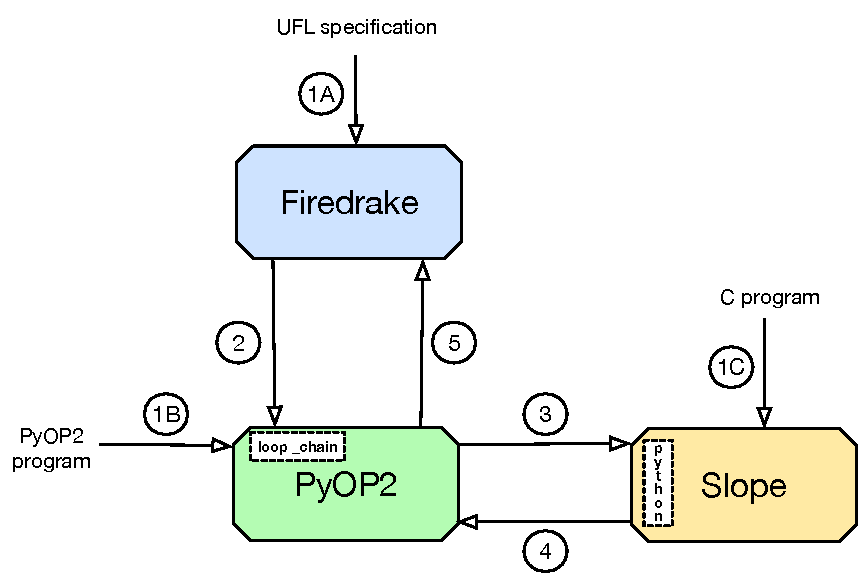
\includegraphics[scale=0.6]{sparsetiling/figures/firedrake-pyop2-slope.pdf}
\caption{Sparse tiling in the Firedrake-PyOP2-SLOPE framework. There are three ways of sparse tiling a loop chain: decorating a Firedrake program (1A), decorating a sequence of loops in a PyOP2 program (1B), writing both the loop chain and the inspector/executor codes explicitly in C through calls to SLOPE (1C). Both (1A) and (1B) use the {\em loop$\_$chain} interface (details in Section~\ref{sec:tiling:lcinterface}). The kernels generated within a {\em loop$\_$chain} are pre-processed in PyOP2 (2) and forwarded to SLOPE through its python interface (3). SLOPE now has access to the loop chain, so it can generate an inspector/executor scheme and return it to PyOP2 (4). The inspector is compiled and executed. The result, a schedule (i.e., the output of Algorithm~\ref{algo:st-inspector}), is cached and used as input to the executor. Each time the same {\em loop$\_$chain} is encountered in a Firedrake/PyOP2 program, the corresponding schedule is reused.}
\label{fig:st-implementation}
\end{figure}

\subsection{SLOPE: a Library for Sparse Tiling Irregular Computations}
\label{sec:tiling:impl-slope}
SLOPE is an open source software that provides an interface to build loop chains and to express inspector/executor schemes for sparse tiling\footnote{SLOPE is a contribution of this thesis and is available at \url{https://github.com/coneoproject/SLOPE}}. 

The loop chain abstraction implemented by SLOPE has been formalized in Section~\ref{sec:tiling:lc-unstruct}. In essence, a loop chain comprises some sets (including the separation into core, boundary, and non-exec regions), maps between sets, and a sequence of loops. Each loop has one or more descriptors specifying what and how different sets are accessed. The example in Listing~\ref{code:tiling-inspector} illustrates the interface exposed by SLOPE. 

SLOPE implements the algorithms in Section~\ref{sec:tiling:inspector}. Further, it provides additional features to estimate the effectiveness and to verify the correctness of sparse tiling:
\begin{description}
\item[VTK file generator] For each tiled loop, a file showing the mesh and the repartition into colored tiles is generated. The file is suitable for visualization in Paraview~\citep{paraview}.
\item[Inspection summary] The inspector returns useful information concerning the sparse tiling process, including: the number and the average size of tiles, the total number of colors used (which can partly explain the performance of a shared-memory parallelization), time spent in the critical inspection phases. 
\end{description}

In the case of shared-memory parallelism, the following sections of code are parallelized through OpenMP:
\begin{itemize}
\item The projection and tiling algorithms; in particular, the loop at line~\ref{algo:st-projection-parallel} of Algorithm~\ref{algo:st-projection} and the loop at line~\ref{algo:st-tiling-parallel} of Algorithm~\ref{algo:st-tiling}).
\item The execution of tiles having the same color; that is, the loops at lines~\ref{algo:st-executor:parallel1} and~\ref{algo:st-executor:parallel2} of Algorithm~\ref{algo:st-executor}.
\end{itemize}


\subsection{PyOP2: Lazy Evaluation and Interfaces}
\label{sec:tiling:lcinterface}
We focus on three relevant aspects of PyOP2: (i) the interface exposed to identify loop chains; (ii) the lazy evaluation mechanism that allows loop chains to be built; (iii) the interaction with SLOPE to build and execute inspector/executor schemes.

To apply sparse tiling to a sequence of loops, PyOP2 provides the {\em loop$\_$chain} interface, as exemplified in Listing~\ref{code:loop-chain-interface}. This interface is exposed to the PyOP2 users, including Firedrake. 

\begin{algorithm}[htpb]
\scriptsize\ttfamily
\SetAlgorithmName{LISTING}{}
\KwSty{with} {\em loop$\_$chain} (name, tile$\_$size, fusion$\_$scheme, ...):\\
~~~~Any Python code here \\
\caption{The {\em loop$\_$chain} interface in PyOP2. The {\tt name} uniquely identifies a loop chain. Other parameters (most of them optional) are useful for performance evaluation (e.g., logging) and performance tuning. The {\tt tile$\_$size} specifies the initial average size for the seed partitions. The {\tt fusion$\_$scheme} allows to specify how to break a long sequence of loops into smaller loop chains, which makes it possible to experiment with a full set of sparse tiling strategies without having to modify the source code.}
\label{code:loop-chain-interface}
\end{algorithm}

PyOP2 exploits lazy evaluation of parallel loops to generate an inspector/executor scheme. The parallel loops encountered during the program execution -- or, analogously, those generated through Firedrake -- are pushed into a queue, instead of being executed immediately. The sequence of parallel loops in the queue is called the {\em trace}. If a dataset $f$ needs to be read, for example because a user wants to inspect its values or a global linear algebra operation needs be performed, the trace is traversed -- from the most recent parallel loop to the oldest one -- and a new sub-trace produced. The sub-trace includes all parallel loops that must be executed to evaluate $f$ correctly. The sub-trace can then be executed or further pre-processed.

All loops in a trace that were created within a {\em loop$\_$chain} scope are sparse tiling candidates. In detail, the interaction between PyOP2 and SLOPE is as follows:
\begin{enumerate}
\item Listing~\ref{code:loop-chain-interface} shows that a {\em loop$\_$chain} defines a new scope. As this scope is entered, a stamp $s_1$ of the trace is generated. This happens ``behind the scenes'', because the {\em loop$\_$chain} is a Python context manager, which can execute pre-specified routines prior and after the execution of the body. As the {\em loop$\_$chain}'s scope is exited, a new stamp $s_2$ of the trace is computed. All parallel loops in the trace generated between $s_1$ and $s_2$ are placed into a sub-trace for pre-processing.
\item The pre-processing consists of two steps: (i) ``simple'' fusion -- consecutive parallel loops iterating over the same iteration space that do not present indirect data dependencies are merged; (ii) generation of a loop chain representation for SLOPE.
\item In (ii), PyOP2 inspects the sequence of loops and translates all relevant data structures (sets, maps, loops) into a format suitable for the SLOPE's Python interface. C code implementing an inspector for the loops in the {\em loop$\_$chain} is returned by SLOPE. PyOP2 compiles and executes this code, which results in an {\em inspection} for the loop chain.
\item A ``software cache'' mapping {\em loop$\_$chain}s to {\em inspection}s is used. This whole process needs therefore be executed only once for a given {\em loop$\_$chain}. 
\item The executor is built in an analogous way to the inspector.
\end{enumerate}


\subsection{Firedrake/DMPlex: the S-depth Mechanism for Extended Halo Regions}
\label{sec:tiling:impl-firedrake}
Firedrake uses DMPlex~\citep{dmplex-cite} to handle meshes. DMPlex is responsible for partitioning, distributing over multiple processes, and locally reordering a mesh. The MPI parallelization is therefore managed through Firedrake/DMPlex.

During the start-up phase, each MPI process receives a contiguous partition of the original mesh from DMPlex. The required PyOP2 sets, which can represent either topological components (e.g., cells, vertices) or function spaces, are created. As explained in Section~\ref{sec:bkg:op2}, these sets distinguish between multiple regions: core, owned, exec, and non-exec. Firedrake initializes the four regions exploiting the information provided by DMPlex. 

To support the loop chain abstraction, Firedrake must be able to allocate arbitrarily deep halo regions. Both Firedrake and DMPlex have been extended to support this feature\footnote{The implementation was mostly carried out by Michael Lange.}. A parameter called {\em S-depth} (the name has historical origins, see for instance~\cite{s-depth-paper}) regulates the extent of the halo regions. A value {\em S-depth} $=n$ indicates the presence of $n$ strips of off-process data elements in each set. The default value is {\em S-depth} $=1$, which enables computation-communication overlap when executing a single loop at the price of a small amount of redundant computation along partition boundaries. This is the default execution model in Firedrake.


\section{Performance Evaluation - Benchmarks}
\label{sec:tiling:benchmarks}
The experimentation of generalized sparse tiling consisted of two phases:

\begin{enumerate}
\item Initially, the technique was tried in two benchmarks: a sparse Jacobi kernel and a proxy unstructured mesh application, originally developed as a demo for the OP2 framework. The objectives of this phase were (i) to explore the impact of generalized sparse tiling on performance, (ii) to characterize the circumstances where the approach is profitable, (iii) to identify the potential limitations of the technique in real applications, (iv) to prototype a compiler. 
\item Then, a real application developed in Firedrake, Seigen (an elastic wave equation solver for seismological problems), was used for systematic performance evaluation. This is presented in Section~\ref{sec:tiling:seigen}. Thanks to its long sequence of loops, Seigen provided a whole suite of sparse tiling benchmark configurations.
\end{enumerate}

In this section, we focus on phase 1. Both benchmarks are written in C. Sparse tiling was introduced manually using a rudimentary version of SLOPE. A previous version of the inspector algorithms presented in this chapter, described in~\cite{st-paper}, was used. As detailed next, one of the major drawbacks of this older inspector was its cost, which grew very rapidly with the number of loops in the chain and the number of distinct datasets accessed. Finally, only shared-memory parallelism via OpenMP was supported. 

In all experiments presented in this section, the optimal tile size (i.e. the one leading to the best execution time) was determined empirically, for each combination of architecture and application. 

\subsection{Sparse Jacobi}

\begin{table}[t]
\centering
\begin{tabulary}{1.0\columnwidth}{c | c | c}
\hline
Matrix name & Execution time reduction $\%$ & Speed-up  \\
\hlineB{4}
{\em ldoor} & 40.34 & 12.11 \\
{\em pwtk} & 38.42 & 11.98 \\
{\em thermal2} & 25.78 & 11.08 \\
{\em xenon2} & 20.15 & 9.53 \\
{\em audikw$\_$1} & 13.42 & 8.70 \\
{\em nd24k} & -151.72 & 3.06 \\
\hline
\end{tabulary}
\caption{Execution time reductions over the original implementation (in percentage) and speed-ups over the single-threaded tiled implementation for the sparse Jacobi solver with 15 threads.}
\label{table:st-jacobi}
\end{table}

The first benchmark was the sparse tiling of a Jacobi sparse matrix solver\footnote{This section is partly extracted from~\cite{st-paper}; the experiments were conducted by Christopher D. Krieger, Catherine Olschanowsky, and Michelle Mills Strout}. Given a sparse matrix $A$, and a vector $\vec{f}$, related by $A\vec{u}=\vec{f}$, each iteration of the sparse Jacobi method produces an approximation to the unknown vector $\vec{u}$. In our experiments, the Jacobi convergence iteration loop is unrolled by a factor of two and the resulting two loops are chained together (1000 iterations of the loop chain was executed). Using a ping-pong strategy, each loop reads from one copy of the $\vec{u}$ vector and writes to the other copy. This experiment was run on an Intel Westmere (dual-socket 8-core Intel Xeon E7-4830 2.13 GHz, 24MB shared L3 cache per socket). The code was compiled using {\tt gcc-4.7.0} with options {\tt -O3 -fopenmp}.

The Jacobi recurrence equation includes a sparse matrix vector multiplication and is representative of a broad class of sparse linear algebra applications. It is also an effective test-bed because different data dependency patterns can be examined simply by using different input matrices. In these experiments, a set of 6 input matrices, drawn from the University of Florida Sparse Matrix Collection~\citep{ST-MatrixMarket}, was used. The matrices were selected so that they would vary in overall data footprint, from 45 MB to 892 MB, and in percentage of non-zeros, from very sparse at 0.0006\% to much more dense at 0.5539\% non-zeros. % values.

Table~\ref{table:st-jacobi} compares the performance of the tiled Jacobi solver to that of a simple blocked version. Both codes use OpenMP \texttt{parallel for} directives to achieve parallelism. The execution time reduction varied from 13$\%$ to 47$\%$ with the exception of the {\em nd24k} matrix, which showed as much as a 1.52x slowdown when sparse tiled. This matrix is highly connected, thus limiting the number of tiles that can be scheduled in parallel. The greater parallelism available under a blocked approach provides more benefit in this case than the performance improvements due to improved locality from full sparse tiling. Overall, speed-ups of between 8 and 12 times over the single-threaded tiled implementation were observed when using 15 threads; a clear outlier is again the {\em nd24k} matrix that did not scale past 3.2 times the single thread performance.

%and typically decreased as threads were added. We believe that this reduction is also related to the parallelism available in the task graph and are investigating methods to mitigate its impact.

The values in Table~\ref{table:st-jacobi} do not include the inspection time necessary to full sparse tile the loop chain. To break even when this cost is considered, the inspector time must be amortized over between 1000 and 3000 iterations of the executor, depending on the specific matrix being solved. We will further elaborate on this aspect in Section~\ref{sec:tiling:bench:conc}.



\subsection{Airfoil}


\begin{table}[t]
\centering
\begin{tabulary}{1.0\columnwidth}{c | c | c | c}
\hline
Architecture & Implementation & Execution time (s) & Speed-up \\
\hlineB{4}
\multirow{3}{*}{Westmere} & {\em omp} & 36.87 & 6.43\\
~ & {\em mpi} & 31.0 & 7.66 \\
~ & {\em tiled} & 26.49 & 8.96 \\
\hline 
\multirow{3}{*}{Sandy Bridge} & {\em omp} & 30.01 & 6.65 \\
~ & {\em mpi} & 24.42 & 8.17 \\
~ & {\em tiled} & 20.63 & 9.67 \\
\hline
\end{tabulary}
\caption{Execution time (in seconds) and speed-ups over the slowest single-threaded implementation for the Airfoil benchmark. Respectively 16 and 24 threads/processes are used on the Sandy Bridge and Westmere machines.}
\label{table:st-airfoil}
\end{table}

The second benchmark was Airfoil, a proxy application designed to represent a class of computations based on the finite volume method~\citep{AIRFOIL}. Three implementations of Airfoil, {\em omp}, {\em mpi} and {\em tiled}, were compared on two shared-memory machines, an Intel Westmere (dual-socket 6-core Intel Xeon X5650 2.66 GHz, 12MB of shared L3 cache per socket) and an Intel Sandy Bridge (dual-socket 8-core Intel Xeon E5-2680 2.00Ghz, 20MB of shared L3 cache per socket). The code was compiled using the Intel \texttt{icc 2013} compiler with optimizations enabled (\texttt{-O3}, \texttt{-xSSE4.2} on the Westmere and \texttt{-xAVX} on the Sandy Bridge).

The Airfoil code consists of a main time loop with 2000 iterations. This loop contains a sequence of four parallel loops that carry out the computation. In this sequence, the first two loops, called $adt$-$calc$ and $res$-$calc$, constitute the bulk of the computation. $Adt$-$calc$ iterates over cells, reads from adjacent vertices and write to a local dataset, whereas $res$-$calc$ iterates over edges and exploits indirect mappings to vertices and cells for incrementing indirect datasets associated to cells. These loops share datasets associated with cells and vertices. Datasets are composed of doubles.
%-precision floating-point values.

The {\em omp} and {\em mpi} versions of Airfoil were implemented in OP2. The effectiveness of these parallelization schemes has been demonstrated in~\cite{op2-main}. The {\em tiled} implementation uses an early version of the SLOPE library (the differences with the inspector algorithms shown in Section~\ref{sec:tiling:inspector} are discussed later) and is based on shared-memory parallelism via OpenMP. We manually unrolled the time loop by a factor of two to be able to tile over 6 loops in total. 

%The OP2 gFST library uses $METIS$~\cite{METIS} for computing a seed partitioning of the mesh vertices.

Table~\ref{table:st-airfoil} shows the runtime reduction achieved by sparse tiling the loop chain on the Westmere and Sandy Bridge architectures. The input unstructured mesh was composed of 1.5 million edges. It is worth noticing that both the {\em omp} and {\em tiled} versions suffer from the well-known NUMA effect as threads are always equally spread across the two sockets. Nevertheless, compared to {\em mpi}, the {\em tiled} version exhibits a peak runtime reduction of 15\% on the Westmere and of 16\% on the Sandy Bridge. 

Results shown for {\em tiled} do not include, however, the inspector overhead. By also including it, the aforementioned improvements over {\em mpi} reduce to roughly 10\% on both platforms. In common with the sparse Jacobi solver, the slow-downs when including the inspection overhead are significant.


\subsection{Outcome}
\label{sec:tiling:bench:conc}

\paragraph{Need for highly optimized inspection}
The inspection overhead can significantly affect sparse tiling. The situation may be even worse in real applications, as usually characterized by longer loop chains, or when the mesh changes over time. This experimental phase led to re-engineering the inspection scheme presented in~\cite{st-paper} into the version described in this chapter. To summarize, the critical differences are: (i) data dependency analysis abstracted to the level of sets, rather than datasets; (ii) optimistic coloring with backtracking in case of conflicts; (iii) parallelization of the projection and tiling routines through the use of inverse maps. 

\paragraph{Need for automation}
The second lesson from this experimentation is that automation is indispensable. Writing the inspector as a sequence of calls to SLOPE is relatively simple, although tedious and error-prone. Integrating the executor is much more complicated, because this requires the rewriting of an entire sequence of loops. This is a severe limitation as it poses an implementation burden on potential users. These considerations led to the multilayer framework detailed in Section~\ref{sec:tiling:automation}, which automatically generates inspector/executor schemes in Firedrake programs. 

\paragraph{Need for distributed-memory support}
The Airfoil experiments highlighted that shared-memory parallelism over multi-socket architectures is drastically affected by the non-uniform memory access (NUMA) issue. The difference in execution time between the OP2 OpenMP and MPI versions is in this sense remarkable. As discussed in~\cite{hydra-op2}, the irregular nature of the computation makes it hard to find systematic solutions to the NUMA issue in the case of pure OpenMP parallelism. The sparse tiled implementation was also purely based on OpenMP, so it suffered from the same problem. This led to the definition of a more general loop chain abstraction (Section~\ref{sec:tiling:lc-unstruct}) and to the introduction of more flexible inspector algorithms (Section~\ref{sec:tiling:inspector}), enabling distributed-memory execution. The MPI and the hybrid OpenMP/MPI execution models are naturally better options for unstructured mesh applications. 

\section{Performance Evaluation - Seigen: an Elastic Wave Equation Solver for Seismological Problems}
\label{sec:tiling:seigen}
In this section, sparse tiling is applied to a computation built on top of Firedrake, Seigen. The performance analysis presented in the following sections is an actual methodological contribution of the thesis. The objectives of this experimentation were to quantify and to motivate in detail the impact of the optimization in a complex, realistic simulation. For this, we executed a large set of experiments on multiple architectures, made use of profilers and analytical tools, and studied the correlation with key simulation parameters, such as the polynomial order and the mesh.

\subsection{Computation}
\label{sec:tiling:seigen:comp}

\subsubsection{The Seismic Model}
Seigen is a novel seismological modelling framework capable of solving the elastic wave equation on unstructured meshes. Exploiting the well-known velocity-stress formulation~\citep{Seigen-3}, the seismic model is expressible as two first-order linear PDEs, which we refer to as {\tt velocity} and {\tt stress}. These governing equations are discretized in space through the discontinuous-Galerkin finite element method. The evolution over time is obtained by using a fourth-order explicit leapfrog scheme based on a truncated Taylor series expansion of the velocity and stress fields. The particular choice of spatial and temporal discretizations has been proven to be non-dissipative~\citep{Seigen-1}. More details can be found in~\cite{Seigen-paper}. Seigen is part of OPESCI, an ecosystem of software for elastic wave modeling~\citep{opesci-project}. 

\subsubsection{Choice of the Test Case}
The Seigen framework has been implemented using Firedrake by Christian Jacobs\footnote{Formerly Imperial College London, now University of Southampton}, along with a set of test cases. In this experimentation, we use the {\tt explosive$\_$source} test case. The test cases may differ in various aspects, such as the initial conditions of the system and the propagation of waves. However, they are all based upon the same seismological model; from a computational viewpoint, this means that, in a time step, the same sequence of loops is executed. Consequently, the performance analysis of {\tt explosive$\_$source} in Section~\ref{sec:tiling:seigen-results} is generalizable to the other test cases. In fact, some of the conclusions will be generalizable to even completely different codes. 

\subsubsection{Implementation}
In a time loop iteration, eight linear systems need be solved, four from {\tt velocity} and four from {\tt stress}. Each solve consists of three macro-steps (see also Section~\ref{sec:bkg:assembly}): assembling a global matrix $A$; assembling a global vector $b$; computing $x$ in the system $Ax = b$. There are two global ``mass'' matrices, one for {\tt velocity} and one for {\tt stress}. Both matrices are
\begin{itemize}
\item Time invariant, so they are assembled before entering the time loop.
\item Block-diagonal, as a consequence of the spatial discretization employed; a block belongs to an element in the mesh. The inverse of a block-diagonal matrix is again block-diagonal and is determined by computing the inverse of each block. The solution of the linear system $Ax = b$, expressible as $x = b A^{-1}$, can therefore be evaluated by looping over the mesh and computing a ``small'' matrix-vector product in each element, where the matrix is a block in $A^{-1}$.
\end{itemize}
Assembling the global vectors reduces to executing a set of loops over mesh entities, particularly over cells, interior facets, and exterior facets. Overall, twenty-five loops are executed in a time loop iteration. Thanks to the hierarchy of ``software caches'' employed by Firedrake, the translation from mathematical syntax into loops is only performed once. 

%Seigen is implemented on top of Firedrake, so most loops are not directly visible in the source code. In particular, all loops arising from the assembly of global vectors (17 in total) are derived automatically from the symbolic specification of {\tt velocity} and {\tt stress}. 

\subsubsection{Application of Sparse Tiling}
Introducing sparse tiling into Seigen was relatively straightforward. Three steps were required: (i) embedding the time stepping loop in a {\em loop$\_$chain} context (see Section~\ref{sec:tiling:lcinterface}), (ii) propagating the relevant user input for performance tuning, (iii) creating a set of {\em fusion schemes}. A fusion scheme establishes which sub-sequences of loops within a {\em loop$\_$chain} will be fused and the respective seed tile sizes. If no fusion schemes were specified, all of the twenty-five loops would be fused using a default tile size. As we shall see, operating with a set of small loop chains and heterogeneous tile sizes is much more effective than fusing long sequences of loops. Hence, specifying multiple fusion schemes is likely to have a direct payoff in performance. As an example, one such scheme treats the loops arising in {\tt velocity} and {\tt stress} as two different loop chains. 

\subsubsection{Validation}
Seigen has several mechanisms to validate the correctness of the seismological model and the test cases. The numerical results of all code versions (with and without tiling) were checked and compared. Paraview was also used to verify the simulation output.

\subsubsection{Parametrization of the Computation}
There are two parameters that we can vary in {\tt explosive$\_$source}: the polynomial order of the method and the input mesh. 

\begin{description}
\item[Polynomial order $q$] We will test the spectrum $q \in \lbrace 1, 2, 3, 4 \rbrace$. To test higher polynomial orders, changes to both the spatial and temporal discretizations would be necessary. For the spatial discretization, the most obvious choice would be tensor product function spaces. However, this functionality is still under development in Firedrake.
\item[Mesh] We use as input a two-dimensional rectangular mesh of fixed size 300$\times$150. We will vary the mesh spacing $h$, which impacts the number of elements in the domain.
\end{description}

\subsubsection{Computational Analysis of the Loops}
We here discuss computational aspects of the twenty-five fusible loops. The following considerations derive from an analytical study of the data movement in the loop chain, extensive profiling through the Intel VTune Amplifier tool~\citep{vtune}, and roofline models (available in~\cite{Seigen-paper}).

\begin{description}
\item[Seigen should benefit from sparse tiling] Not only does data reuse arise within single loops (e.g., by accessing vertex coordinates from adjacent cells), but also across consecutive loops, through indirect data dependencies. This makes Seigen a natural fit for sparse tiling. 

\item[Data reuse across solvers] Eight ``solver'' loops perform matrix-vector multiplications in each mesh element. It is well established that linear algebra operations of this kind are memory-bound. Four of these loops arise from {\tt velocity}, the others from {\tt stress}. There is significant data reuse amongst the four {\tt velocity} loops and amongst the four {\tt stress} loops, since the same blocks in the global inverse matrices are accessed. We hypothesize performance gains if these loops were fused through sparse tiling.

\item[Exterior facet loops have negligible cost] Three loops implement the boundary conditions of the variational problems by iterating over the exterior mesh facets. The impact of these loops on the completion time is negligible, since their iteration space is order of magnitude smaller than that of cells and facets loops.

\item[Data reuse across cells and facets loops] Six loops iterate over the interior mesh facets to compute so called facet integrals. Facet integrals ensure the propagation of information between adjacent cells in discontinuous-Galerkin methods. The operational intensity of these loops is much lower than that of cell loops, and memory-boundedness is expected. Consecutive facet and cell integral loops share fields, which creates cross-loop data reuse opportunities. Again, sparse tiling might play a key role in transforming this data reuse into data locality.

\item[Optimizing the operational intensity] All computational kernels generated in Seigen are optimized through COFFEE (Chapters~\ref{ch:optimality},~\ref{ch:lowlevelopt},~\ref{ch:coffee}). In essence: (i) the operation count is minimized by restructuring expressions and loop nests; (ii) auto-vectorization opportunities are created by using array padding and by enforcing data alignment.
\end{description}



\subsection{Setup and Reproducibility}

\subsubsection{Fusion Schemes and Attempted Optimizations}
\label{sec:tiling:seigen:opts}
The generality of the sparse tiling algorithms, the flexibility of the {\em loop$\_$chain} interface, and the {\em S-depth} mechanism made it possible to experiment with a variety of fusion schemes without changes to the source code. 

Five fusion schemes were devised, based on the following criteria: (i) amount of data reuse, (ii) amount of redundant computation over the boundary region, (iii) memory footprint (the larger, the smaller the tile size to fit in cache). The fusion schemes are summarized in Table~\ref{table:seigen-fusion-schemes}, while the full specification is available at~\cite{seigen-code}.

\begin{table}[htpb]
\footnotesize
\centering
\makebox[\textwidth][c]
{
\begin{tabulary}{1.0\columnwidth}{M{0.9cm} | M{1.7cm} | M{8.3cm} | M{1.0cm} N}
\hline
Fusion scheme & Number of loop chains & Criterion & {\em S-depth}  \\
\hlineB{4}
{\tt fs1} & 3 & Fuse {\tt velocity} cells and facets loops & 2 & \\[5pt] \hline
{\tt fs2} & 8 & {\tt fs1} and fuse {\tt stress} cells and facets loops & 2 & \\[5pt] \hline
{\tt fs3} & 6 & {\tt fs2} and fuse some solver loops & 2 & \\[5pt] \hline
{\tt fs4} & 3 & More aggressive than {\tt fs2} & 3 & \\[5pt] \hline
{\tt fs5} & 2 & Maximize locality in the {\tt velocity} and {\tt stress} loop chains & 4 & \\[5pt] \hline
\end{tabulary}
}
\caption{Summary of the fusion schemes adopted in Seigen. The {\em S-depth} column represents the number of off-process cell layers.}
\label{table:seigen-fusion-schemes}
\end{table}

Furthermore, several optimizations, applicable to all fusion schemes, were tried.

\begin{description}
\item[Global and local maps] Algorithm~\ref{algo:st-inspector} computes so called local maps to avoid an extra level of indirection in the executor. We regard this as a {\it potential optimization}. Although no data reuse is available for the local maps (each fused loop has its own local maps), there might be benefits from improved hardware prefetching and memory latency. We will experiment with both global (i.e., original, as constructed by Firedrake and provided in the loop chain specification) and local (i.e., computed by SLOPE) maps. 
%The runs using local maps will be represented with the suffix {\tt lm}.

\item[Tile shape] The seed loop partitioning and the mesh numbering determine the tile shape. The simplest way of creating tiles consists of ``chunking'' the seed iteration space every $ts$ iterations, with $ts$ being the initial tile size (see Section~\ref{sec:tiling:inspector}). The {\tt chunk} partitioning inherits the original mesh numbering. In Firedrake, and therefore in Seigen, meshes are renumbered during initialization applying the reverse Cuthill–McKee (RCM) algorithm. Using {\tt chunk} partitioning on top of an RCM-renumbered mesh has the effect of producing thin, rectangular tiles. This affects tile expansion, as a large proportion of elements lie on the tile border. There are potential solutions to this problem. The most promising would consist of using a Hilbert curve, rather than RCM, to renumber the mesh. This would lead to more regular polygonal tiles when applying {\tt chunk} partitioning. Unfortunately, Hilbert curves are at the moment not supported in Firedrake. An alternative consists of partitioning the seed iteration space with a library like METIS~\citep{METIS} before applying RCM. As we shall see, this approach is not exempt from side effects.

\item[Software prefetching] In a loop, there are usually more than a single stream of memory accesses amenable to hardware prefetching (e.g., accesses to the indirection maps; direct accesses to data values; indirect accesses to data values if the mesh has a good numbering). Sparse tiling, unfortunately, impairs hardware prefetching for two reasons: (i) the virtual addresses streams are considerably shorter; (ii) tile expansion introduces irregularities in these streams. Software prefetching can be used together with hardware prefetching to minimize memory stalls. PyOP2 and SLOPE have been extended to emit intrinsics instructions for prefetching the iteration $i$'s maps and data values while executing iteration $i-1$. 
%The runs using software prefetching will be represented with the suffix {\tt sw-pre}.

\item[Extended boundary region] The special non-exec tile $T_{ne}$ (see Sections~\ref{sec:tiling:examples} and~\ref{sec:tiling:inspector}) reduces the amount of redundant computation in long loop chains by expanding over boundary tiles. There are two ways of creating $T_{ne}$: either an extra layer of data is added to the boundary region (e.g., see Figure~\ref{fig:st-mpi-init}) or during inspection, by searching for mesh boundaries. The current implementation only supports the first option. Manually deriving $T_{ne}$ would be not only algorithmically complex, but also potentially very expensive.
\end{description}



\subsubsection{Systems Configuration and Execution Modes}
Extensive experimentation was performed on two Intel architectures, whose specification is reported in Table~\ref{table:seigen-setup}. 

\begin{table}[htpb]
\scriptsize
\makebox[\textwidth][c]
{
\begin{tabulary}{1.2\textwidth}{M{2.0cm} V{4} M{4.4cm} | M{5.4cm} N}
\hline
System & Erebus & CX1-Ivy \\
\hlineB{4}
Node & 1x4-core Intel I7-2600 3.4GHz & 2x20-core Intel Xeon E5-2660 2.20GHz & \\[15pt] \hline
DRAM & 16 GB & 64 GB & \\[5pt] \hline
STREAM performance & 18.5 GB/s (4.6 GB/s per core)&  92.0 GB/s (4.6 GB/s per core) & \\[15pt] \hline
Cache hierarchy & \shortstack{L1=32KB, L2=256KB, L3=8MB\\ L3 is shared} & \shortstack{L1=32KB, L2=256KB, L3=25MB\\L3 is shared per socket (50MB total)} & \\[15pt] \hline
Compilers & Intel {\tt icc} 16.0.2 & Intel {\tt icc} 15.1 & \\[5pt] \hline
Compiler flags & {\tt -O3 -xHost -ip} & {\tt -O3 -xHost -ip} & \\[5pt] \hline
MPI version & Open MPI 1.6.5 & Intel MPI 5.1 & \\[5pt] \hline
MPI options & {\tt --bind-to-core} & \shortstack{{\tt I$\_$MPI$\_$DEVICE ssm}\\{\tt I$\_$MPI$\_$PIN yes}\\{\tt I$\_$MPI$\_$PIN$\_$MODE lib}\\{\tt I$\_$MPI$\_$PIN$\_$PROCESSOR$\_$LIST map=bunch}} & \\[35pt] \hline
\end{tabulary}
}
\caption{Systems specification.}
\label{table:seigen-setup}
\end{table}

Support for shared-memory parallelism is discontinued in Firedrake, so only distributed-memory parallelism was tested. MPI processes were pinned to cores. The hyperthreading technology was not used. Erebus and CX1-Ivy were unstressed and exclusive access had been obtained when the runs were performed. 

\subsubsection{Meshes}
The (average) number of degrees of freedom $d$ assigned to a process mainly depends on the polynomial order $q$, the mesh spacing $h$ and the number of cores $n$ in a node. Meshes are chosen such that: (i) $d$ fits in main memory; (ii) $d$ exceeds the last level of cache; (iii) ${<}d,\ q,\ h{>}$ ensure convergence of the simulation. A summary of the meshes used for experimentation is provided in Table~\ref{table:seigen-meshes}.

\begin{table}[htpb]
\footnotesize
\centering
\begin{tabulary}{1.0\columnwidth}{c V{4} c V{4} c | c | c | c V{4} c | c | c | c N}
\hline
\multirow{2}{*}{System} & \multirow{2}{*}{$h$}  & \multicolumn{4}{c V{4}}{$d$ {\tt velocity}} & \multicolumn{4}{c}{$d$ {\tt stress}} & \\[4pt] \cline{3-11}
 & & $q=1$ & $q=2$ & $q=3$ & $q=4$ & $q=1$ & $q=2$ & $q=3$ & $q=4$ & \\[4pt]
\hlineB{4}
\rule{0pt}{3ex}  \multirow{2}{*}{\shortstack{Erebus\\$(n=4)$}} & 1.0 & 138k & 276k & 460k & 690k & 276k & 552k & 920k & 1379k \\[4pt]
& 1.2 & 96k & 192k & 320k & 480k & 192k & 385k & 641k & 961k \\[4pt]
\hline
\rule{0pt}{3ex}  \multirow{2}{*}{\shortstack{CX1-Ivy\\$(n=20)$}} & 0.6 & 78k & 157k & 262k & 393k & 157k & 314k & 525k & 787k  \\[4pt]
& 0.8 & 44k & 89k & 149k & 223k & 89k & 178k & 298k & 447k \\[4pt]
\hline
\end{tabulary}
\caption{Summary of the meshes used for single-node experimentation in Seigen. $d$ is the average number of degrees of freedom assigned to a process for a given variational form.}
\label{table:seigen-meshes}
\end{table}



\subsubsection{Timing Criteria}
For each experiment, we collect three measurements.

\begin{description}
\item[Overall completion time (OT)] Used to compute the maximum application speed-up when sparse tiling is applied. 
\item[Average compute time (ACT)] Sparse tiling impacts the kernel execution time by increasing data locality. Communication is also influenced, especially in aggressive fusion schemes: the rounds of communication decrease, while the data volume exchanged may increase. ACT isolates the gain due to increased data locality from (i) the communication cost and (ii) any other action performed in Firedrake (executing Python code) between the invocation of kernels. This value is averaged across the processes.
\item[Average compute and communication time (ACCT)] As opposed to ACT, the communication cost is also included in ACCT. By comparing ACCT and ACT, the communication overhead can be derived. 
\end{description}
As we shall see, all of these metrics will be essential for a complete understanding of the sparse tiling performance. It is true that for much larger meshes ACT and ACCT should converge to OCT, but such an experimentation is not feasible as it would require weeks, possibly months, of compute time.

To collect OT, ACT and ACCT, the following configuration was adopted.
\begin{itemize}
\item All experiments were executed with ``warm cache''; that is, with all kernels retrieved directly from the Firedrake's cache, so code generation and compilation times are not counted.
\item All of the non-tiled {\tt explosive$\_$source} tests were repeated three times. The sparse tiling search space is big (the product of all $q$, fusion schemes, tile sizes, meshes and a set of additional optimizations) and some tests can last longer than a hour, so for practical reasons the tiled {\tt explosive$\_$source} tests were repeated two times, instead of three. The minimum times are reported (negligible variance).
\item The cost of global matrix assembly -- an operation that takes place before entering the time loop -- {\it is not} included in OT. Firedrake needs be extended to assemble block-diagonal matrices directly into vectors (an entry in the vector would represent a matrix block). Currently, this is instead obtained in two steps: first, by assembling into a CSR matrix; then, by explicitly copying the diagonal into a vector (a Python operation). The assembly per se never takes more than 3 seconds, so it is reasonable to exclude this temporary overhead from our timing.
\item The inspection cost due to sparse tiling {\it is} included in OT.
\item Extra costs were minimized: no check-pointing, only two I/O sessions (at the beginning and at the end of the computation), and minimal logging.
\item The time loop has a fixed duration $T$, while the time step depends on the mesh spacing. In essence, finer meshes require proportionately smaller time steps to ensure convergence. Furthermore, $T$ cannot be reduced arbitrarily, which makes the performance exploration longer. A (prolonged) transitory period $P$ is necessary so that the waves fully propagate across the domain. During $P$, the data movement is greatly reduced as most data values are unchanged. The effects of sparse tiling become evident only if $T$ is sufficiently longer than $P$, so complete simulations had to be executed.
\end{itemize}



\subsection{Results and Analysis}
\label{sec:tiling:seigen-results}
In this section, we report on hundreds of experiments aimed at quantifying the performance improvements obtainable in Seigen when sparse tiling is applied. Using the {\tt explosive$\_$source} test case, we explore a large set of parameters, which includes polynomial order, mesh, node architecture, fusion scheme, and many others. A generic instance of {\tt explosive$\_$source} optimized with sparse tiling will be referred to as a ``tiled version'', otherwise the term ``original version'' will be used. The structure of this section is as follows:

\begin{enumerate}
\item We start with an overview of the maximum speed-ups obtained through sparse tiling. Some preliminary observations are made.
\item We delineate the structure of the search space exploration for determining the optimal sparse tiling version. 
\item We motivate, in detail, through plots and the {\it loop chain analyzer} tool, the performance of the various fusion schemes and optimizations attempted.
\item We provide further evidence from profiler reports.
\item We comment on the performance bottlenecks introduced by sparse tiling.
\end{enumerate}

%A generalization of this study -- in particular, of the factors limiting sparse tiling -- to different programs is provided. 

\subsubsection{Summary of the Attained Speed-ups}
The times that we report below derive from runs at maximum degree of parallelism (i.e., 1 MPI process per physical core). The benefits from sparse tiling (if any) tend to be negligible in other types of runs (e.g., sequential runs). As elaborated in the following sections, this is a consequence of three factors: (i) the memory access latency is only marginally affected when a large proportion of bandwidth is available to the processes; (ii) hardware prefetching is impaired by the small iteration space of tiles; (iii) TLB misses are more frequent due to tile expansion.

Table~\ref{table:seigen-speedups} reports the completion times (OT) for the original and tiled versions of Seigen, on both Erebus and CX1-Ivy. For each node architecture, polynomial order $q$ and mesh, the best tiled version time is reported; the search space exploration that led to this number will be detailed in the next section. The speed-up for OT achieved through sparse tiling is indicated as $\Omega^{OT}$. Tables~\ref{table:seigen-speedups-ACT} and~\ref{table:seigen-speedups-ACCT} show analogous information for ACT and ACCT.

\begin{table}[b]
\large
\centering
%\STautoround*{2}
\begin{spreadtab}{{tabular}{c V{4} c V{4} M{0.7cm} V{4} M{2.8cm} | M{2.8cm} V{4} M{1.5cm}}}
\hline
@ System & @ $h$ & @ $q$ & @ OT (s) & @ OT tiled (s) & @ $\Omega^{OT}$  \\
@ \hlineB{4}
@ \multirow{8}{*}{\shortstack{Erebus\\$(n=4)$}} & @ \multirow{4}{*}{$1.0$} & @ 1 & 687 & 596 & round([-2,0]/[-1,0],2) \\ 
@ & @ & @ 2 & 1453 & 1200 &round([-2,0]/[-1,0],2)  \\ 
@ & @ & @ 3 & 3570 & 2847 & round([-2,0]/[-1,0],2) \\
@ & @ & @ 4 & 7057 & 5827 & round([-2,0]/[-1,0],2) \\
@\cline{2-6}
@ & @ \multirow{4}{*}{$1.2$} & @ 1 & 419 & 365 & round([-2,0]/[-1,0],2) \\ 
@ & @ & @ 2 & 870 & 715 & round([-2,0]/[-1,0],2)  \\ 
@ & @ & @ 3 & 1937 & 1549 & round([-2,0]/[-1,0],2) \\
@ & @ & @ 4 & 4110 & 3390 & round([-2,0]/[-1,0],2) \\
@\hlineB{4}
@ \multirow{8}{*}{\shortstack{CX1-Ivy\\$(n=20)$}} & @ \multirow{4}{*}{$0.6$} & @ 1 & 859 & 813 & round([-2,0]/[-1,0],2) \\ 
@ & @ & @ 2 &  1712 & 1585 & round([-2,0]/[-1,0],2)  \\ 
@ & @ & @ 3 & 3680 & 3378 & round([-2,0]/[-1,0],2) \\
@ & @ & @ 4 & 8051 & 6962 & round([-2,0]/[-1,0],2) \\
@\cline{2-6}
@ & @ \multirow{4}{*}{$0.8$} & @ 1 & 396 & 390 & round([-2,0]/[-1,0],2) \\ 
@ & @ & @ 2 & 770 & 721 & round([-2,0]/[-1,0],2)  \\ 
@ & @ & @ 3 & 1562 & 1457 & round([-2,0]/[-1,0],2) \\
@ & @ & @ 4 & 3263 & 2931 & round([-2,0]/[-1,0],2) \\
@ \hline
\end{spreadtab}
\caption{Comparing the Seigen completion time OT on Erebus (number of processes $n=4$) and CX1-Ivy ($n=20$).}
\label{table:seigen-speedups}
\end{table}



\begin{table}[htpb]
\large
\centering
%\STautoround*{2}
\begin{spreadtab}{{tabular}{c V{4} c V{4} M{0.7cm} V{4} M{2.8cm} | M{2.8cm} V{4} M{1.5cm}}}
\hline
@ System & @ $h$ & @ $q$ & @ ACT (s) & @ ACT tiled (s) & @ $\Omega^{ACT}$  \\ 
@ \hlineB{4}
@ \multirow{8}{*}{\shortstack{Erebus\\$(n=4)$}} & @ \multirow{4}{*}{$1.0$} & @ 1 & 533 & 455 & round([-2,0]/[-1,0],2) \\ 
@ & @ & @ 2 & 1252 & 999 &round([-2,0]/[-1,0],2)  \\ 
@ & @ & @ 3 & 3255 & 2549 & round([-2,0]/[-1,0],2) \\
@ & @ & @ 4 & 6585 & 5401 & round([-2,0]/[-1,0],2) \\
@\cline{2-6}
@ & @ \multirow{4}{*}{$1.2$} & @ 1 & 313 & 267 & round([-2,0]/[-1,0],2) \\ 
@ & @ & @ 2 & 729 & 579 & round([-2,0]/[-1,0],2)  \\ 
@ & @ & @ 3 & 1746 & 1360 & round([-2,0]/[-1,0],2) \\
@ & @ & @ 4 & 3837 & 3127 & round([-2,0]/[-1,0],2) \\
@\hlineB{4}
@ \multirow{8}{*}{\shortstack{CX1-Ivy\\$(n=20)$}} & @ \multirow{4}{*}{$0.6$} & @ 1 & 484 & 448 & round([-2,0]/[-1,0],2) \\ 
@ & @ & @ 2 &  1149 & 1015 & round([-2,0]/[-1,0],2)  \\ 
@ & @ & @ 3 & 2740 & 2471 & round([-2,0]/[-1,0],2) \\
@ & @ & @ 4 & 6354 & 5423 & round([-2,0]/[-1,0],2) \\
@\cline{2-6}
@ & @ \multirow{4}{*}{$0.8$} & @ 1 & 191 & 175 & round([-2,0]/[-1,0],2) \\ 
@ & @ & @ 2 & 486 & 434 & round([-2,0]/[-1,0],2)  \\ 
@ & @ & @ 3 & 1159 & 1068 & round([-2,0]/[-1,0],2) \\
@ & @ & @ 4 & 2654 & 2307 & round([-2,0]/[-1,0],2) \\
@ \hline
\end{spreadtab}
\caption{Comparing the Seigen average compute time ACT on Erebus (number of processes $n=4$) and CX1-Ivy ($n=20$).}
\label{table:seigen-speedups-ACT}
\end{table}



\begin{table}[htpb]
\large
\centering
%\STautoround*{2}
\begin{spreadtab}{{tabular}{c V{4} c V{4} M{0.7cm} V{4} M{2.8cm} | M{2.8cm} V{4} M{1.5cm}}}
\hline
@ System & @ $h$ & @ $q$ & @ ACCT (s) & @ ACCT tiled (s) & @ $\Omega^{ACCT}$  \\
@ \hlineB{4}
@ \multirow{8}{*}{\shortstack{Erebus\\$(n=4)$}} & @ \multirow{4}{*}{$1.0$} & @ 1 & 581 & 503 & round([-2,0]/[-1,0],2) \\
@ & @ & @ 2 & 1334 & 1071 &round([-2,0]/[-1,0],2)  \\
@ & @ & @ 3 & 3438 & 2712 & round([-2,0]/[-1,0],2) \\
@ & @ & @ 4 & 6881 & 5661 & round([-2,0]/[-1,0],2) \\
@\cline{2-6}
@ & @ \multirow{4}{*}{$1.2$} & @ 1 & 340 & 293 & round([-2,0]/[-1,0],2) \\
@ & @ & @ 2 & 776 & 618 & round([-2,0]/[-1,0],2)  \\
@ & @ & @ 3 & 1827 & 1437 & round([-2,0]/[-1,0],2) \\
@ & @ & @ 4 & 3987 & 3265 & round([-2,0]/[-1,0],2) \\
@\hlineB{4}
@ \multirow{8}{*}{\shortstack{CX1-Ivy\\$(n=20)$}} & @ \multirow{4}{*}{$0.6$} & @ 1 & 638 & 586 & round([-2,0]/[-1,0],2) \\
@ & @ & @ 2 &  1468 & 1336 & round([-2,0]/[-1,0],2) \\
@ & @ & @ 3 & 3398 & 3087 & round([-2,0]/[-1,0],2) \\
@ & @ & @ 4 & 7745 & 6649 & round([-2,0]/[-1,0],2) \\
@\cline{2-6}
@ & @ \multirow{4}{*}{$0.8$} & @ 1 & 230 & 247 & round([-2,0]/[-1,0],2) \\
@ & @ & @ 2 & 603 & 543 & round([-2,0]/[-1,0],2) \\
@ & @ & @ 3 & 1378 & 1278 & round([-2,0]/[-1,0],2) \\
@ & @ & @ 4 & 3061 & 2730 & round([-2,0]/[-1,0],2) \\
@ \hline
\end{spreadtab}
\caption{Comparing the Seigen average compute and communication time ACCT on Erebus (number of processes $n=4$) and CX1-Ivy ($n=20$).}
\label{table:seigen-speedups-ACCT}
\end{table}

Based on these tables, some preliminary observations can be made.
\begin{itemize}
\item Despite a similar amount of available bandwidth per core, an improved core architecture and a better cache hierarchy (see Table~\ref{table:seigen-setup}) the speed-ups on CX1-Ivy are generally not as high as on Erebus. Profiling through Intel VTune showed that the proportion of time spent on executing compute-bound loops is higher on CX1-Ivy than on Erebus, but further investigation is required to explain this behaviour. It would be interesting to carry out a similar performance exploration on a many-core architecture, like Intel's Knights Landing, characterized by less powerful cores and a completely different memory system. Testing on multi-node systems is also high priority future work, as this will increase the pressure on the memory system due to inter-node communication. 

\item The performance improvements are generally greater than 1.10$\times$, and often exceed 1.20$\times$. In light of the limiting factors discussed in the next sections, this is a promising result. While some of these limiting factors are inherent in Seigen and sparse tiling, others are simply due to shortcomings of the current implementation. We therefore envisage ample space for improvements. $\Omega^{ACT}$ and $\Omega^{ACCT}$ are, as expected, higher than $\Omega^{OT}$. ACT, in particular, tells us that the benefits from the relieved memory pressure outweigh the redundant computation overhead.

\item The performance improvements tend to increase with $q$. This is remarkable, but not surprising. The memory footprint of a loop grows with $q$, hence all negative effects such as impaired hardware prefetching and TLB misses (properly documented in the next sections) caused by sparse tiling become less notable. This trend can be appreciated in all problem instances. 
\end{itemize}



%gain grows with q
%The search for the best tiled version is described in the next section. 

\subsubsection{Structure of the Search Space Exploration}
The best tiled version for a specific problem instance was determined empirically, trying all possible combinations out of a set of parameters. The space of parameters was described in Section~\ref{sec:tiling:seigen:opts} and is summarized below.

\begin{description}
\item[Fusion scheme] Five fusion schemes ({\tt fs$X$, $X \in \lbrace 1, 2, 3, 4, 5\rbrace$}) were studied (see Table~\ref{table:seigen-fusion-schemes}).
\item[Seed tile size] For each {\tt fs} and $q$, three or four tile sizes were tested. Four tile sizes were used with $q \in \lbrace 1, 2\rbrace$. The tile sizes were chosen to maximize the likelihood of fitting in L2 or L3 cache. A less extensive experimentation with ``more adverse'' tile sizes showed that: (i) a very small value causes dramatic slow-downs (up to 8$\times$ slower than the original versions); (ii) larger values cause proportionately greater slow-downs.
\item[Indirection maps] Both local and global maps were tested.
\item[Partitioning] Two partitioning strategies were tested: {\tt chunk} and {\tt metis}.
\item[Extended boundary region] All experiments were repeated with and without the extended boundary region optimization discussed in Section~\ref{sec:tiling:seigen:opts}.
%Two fusion schemes out of six may benefit from an extended boundary region to minimize redundant computation.
\end{description}

Software prefetching and a small set of prefetch distances were also tested in a few instances of {\tt explosive$\_$source}, but no significant changes to the execution times were observed. It was decided, therefore, to exclude this parameter from the search space; this made it possible to execute the whole test suite in slightly less than five days. 

An {\tt explosive$\_$source} instance is determined by three parameters:

\begin{description}
\item[Node architecture] The two systems shown in Table~\ref{table:seigen-setup} were used.
\item[Polynomial order] $q \in \lbrace 1, 2, 3, 4\rbrace$.
\item[Mesh] The meshes shown in Table~\ref{table:seigen-meshes} were used (two meshes for each node architecture).
\end{description}

We experimented with $2 \times 4 \times 2 = 16$ {\tt explosive$\_$source} instances. For each of these instances, we tested the original Seigen version and a set of tiled versions. When $q \in \lbrace 1, 2 \rbrace$, a set of tiled version consists of $5 \times 4 \times 2 \times 2 \times 2 = 160$ instances (otherwise, with $q \in \lbrace 3, 4 \rbrace$, the instances are 120). In total, we executed $8 \times (160 + 1) + 8 \times (120 + 1) = 2256$ versions of Seigen on single node. 

Given the large number of problem instances, the results of the search space exploration are organized as follows. We show one plot for each of the sixteen {\tt explosive$\_$source} instances. A plot illustrates the search space exploration for given node architecture, $h$ and $q$. The ACCT of the original version and a subset of tiled versions is reported on the y-axis. To make the plots readable, the impact of (i) local/global indirection maps, (ii) normal/extended boundary region, (iii) {\tt chunk}/{\tt metis} partitioning strategies are only discussed qualitatively. Fortunately, it is very straightforward to draw general conclusions about the effect of these optimizations. The raw execution times are available at~\cite{phd-thesis-repo}.

\subsubsection{Outcome of the Search Space Exploration}

\begin{figure}[htpb]
\captionsetup{font=scriptsize}
\caption{Search space exploration on Erebus with $n=4$ MPI processes. Two meshes ($h \in \lbrace 1.0, 1.2\rbrace$) and four polynomial orders ($q \in \lbrace 1, 2, 3 ,4\rbrace$) are shown. Each plot shows the average compute and communication time (ACCT, y-axis) of five fusion schemes and the original version. The seed tile size of a loop chain in an {\tt fs}, in terms of seed loop iterations, is the product of the ``tile size factor'' (x-axis) and a pre-established multiplier (an integer in the range $[1, 4]$; full list at~\cite{seigen-code}). With tiling, global maps, {\tt chunk} partitioning, and the extended boundary region optimization are used.}

\par\bigskip
\par\medskip

\begin{subfigure}[]{1.02\textwidth}
~~~~~~~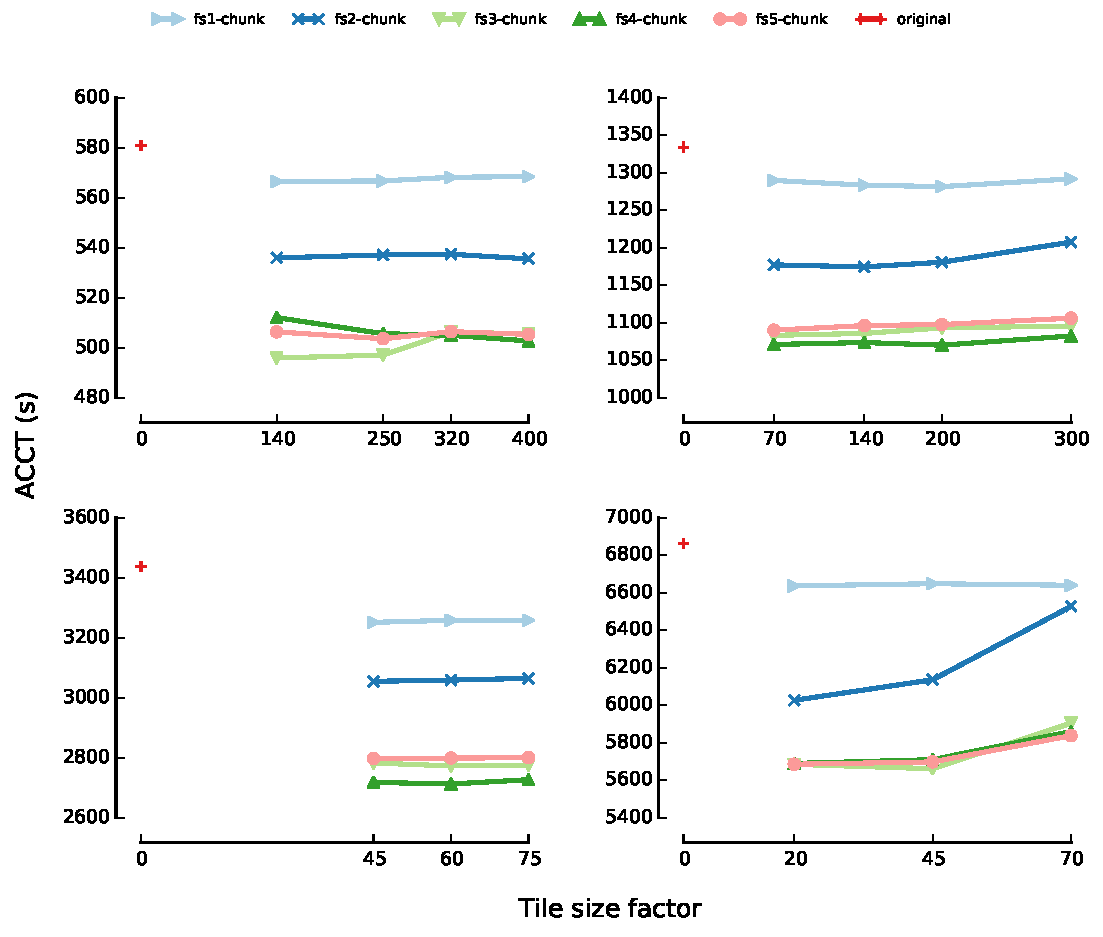
\includegraphics[scale=0.55]{sparsetiling/perf-eval/summary/grid_erebus_plexmesh_h10_mpi.pdf}
\caption{$h = 1.0$.}
\label{fig:st-erebus-expl-h10}
\end{subfigure}%

\par\medskip

\begin{subfigure}[]{1.02\textwidth}
~~~~~~~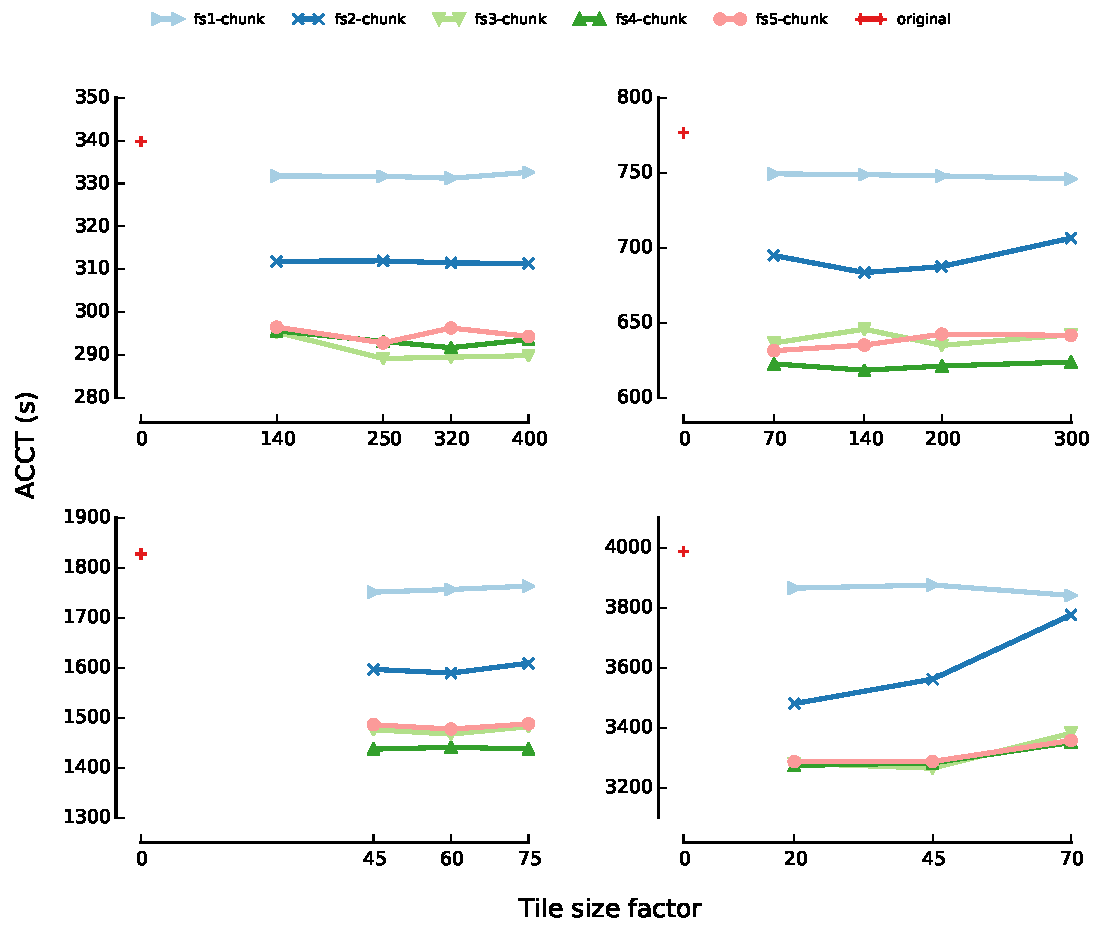
\includegraphics[scale=0.55]{sparsetiling/perf-eval/summary/grid_erebus_plexmesh_h12_mpi.pdf}
\caption{$h = 1.2$.}
\label{fig:st-erebus-expl-h12}
\end{subfigure}%


\label{fig:st-erebus-expl}
\end{figure}


\begin{figure}[htpb]
\captionsetup{font=scriptsize}
\caption{Search space exploration on CX1-Ivy with $n=20$ MPI processes. Two meshes ($h \in \lbrace 0.6, 0.8\rbrace$) and four polynomial orders ($q \in \lbrace 1, 2, 3 ,4\rbrace$) are shown. Each plot shows the average compute and communication time (ACCT, y-axis) of five fusion schemes and the original version. The seed tile size of a loop chain in an {\tt fs}, in terms of seed loop iterations, is the product of the ``tile size factor'' (x-axis) and a pre-established multiplier (an integer in the range $[1, 4]$; full list at~\cite{seigen-code}). With tiling, global maps, {\tt chunk} partitioning, and the extended boundary region optimization are used.}

\par\bigskip
\par\medskip

\begin{subfigure}[]{1.02\textwidth}
~~~~~~~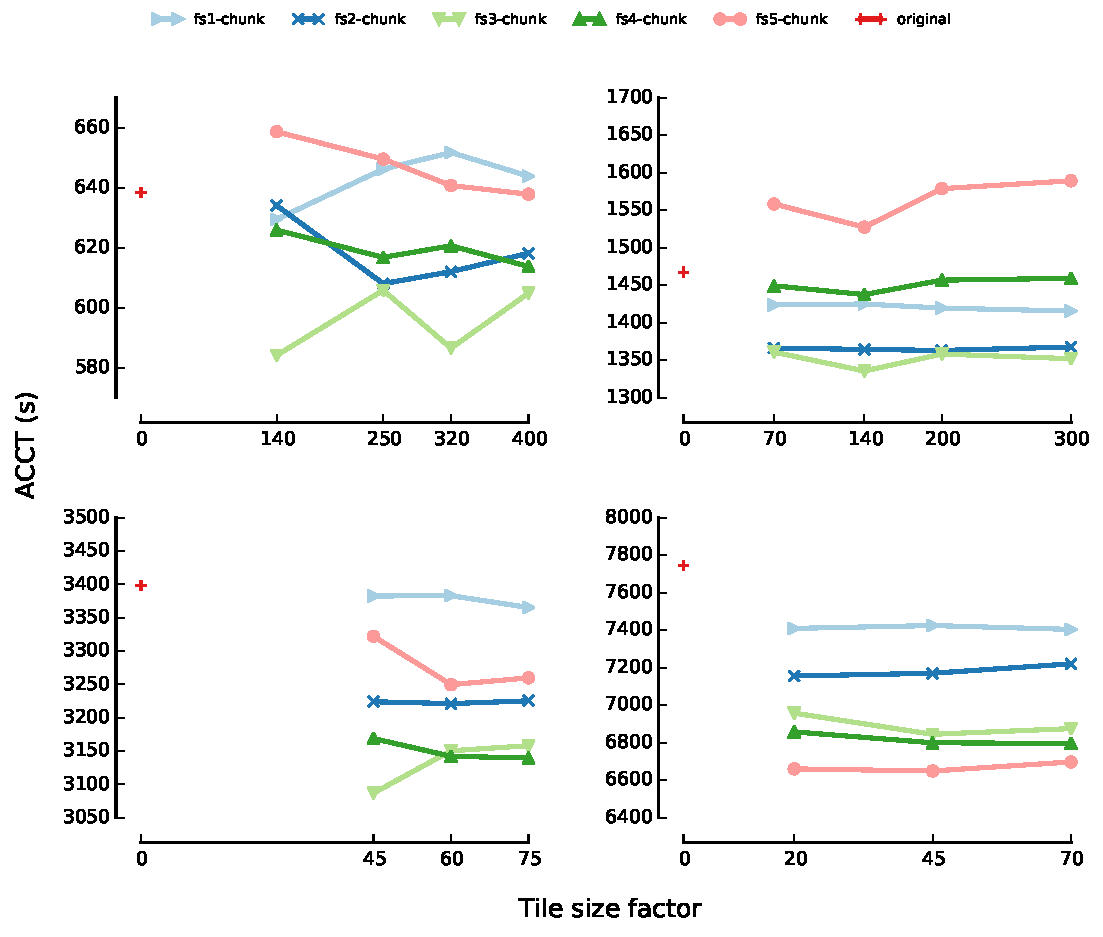
\includegraphics[scale=0.55]{sparsetiling/perf-eval/summary/grid_cx1-ivy_plexmesh_h06_mpi.pdf}
\caption{$h = 0.6$.}
\label{fig:st-cx1-expl-h06}
\end{subfigure}%

\par\medskip

\begin{subfigure}[]{1.02\textwidth}
~~~~~~~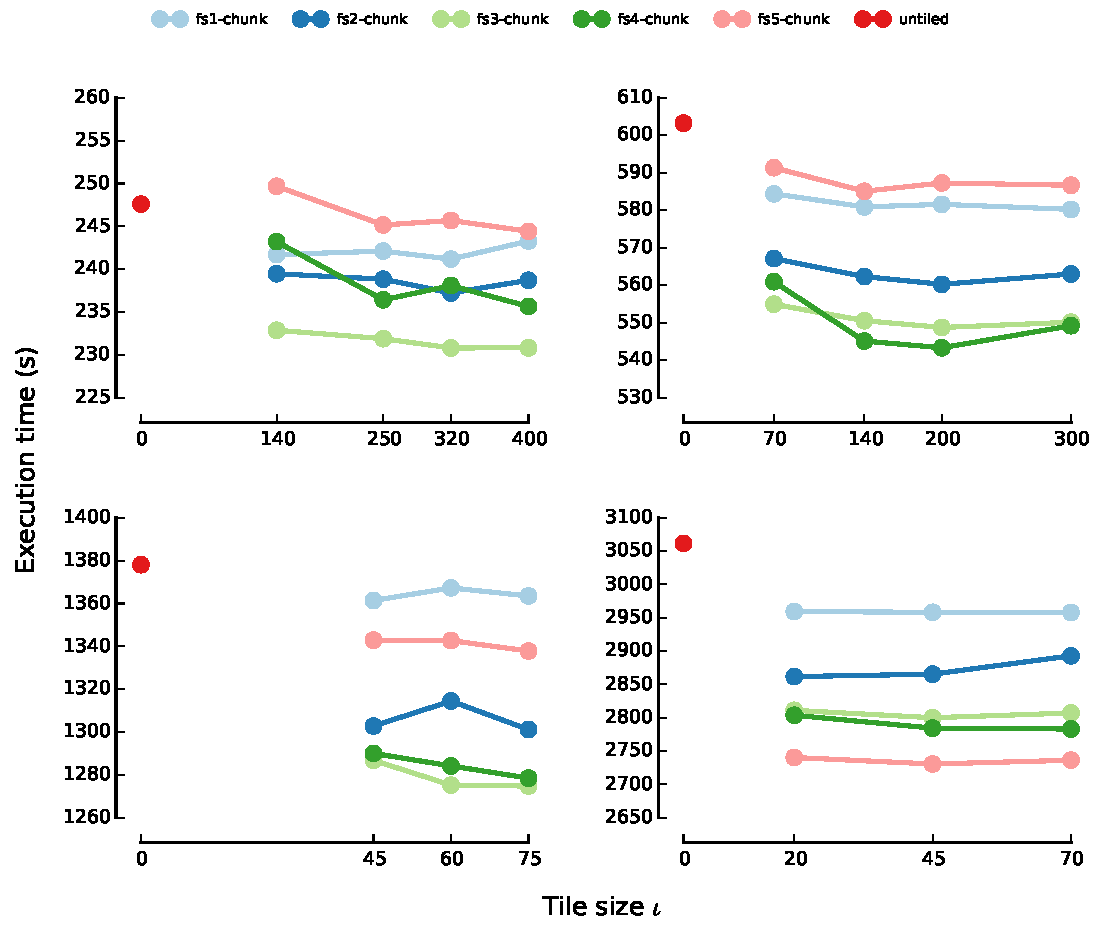
\includegraphics[scale=0.55]{sparsetiling/perf-eval/summary/grid_cx1-ivy_plexmesh_h08_mpi.pdf}
\caption{$h = 0.8$.}
\label{fig:st-cx1-expl-h08}
\end{subfigure}%

\label{fig:st-cx1-expl}
\end{figure}


PyOP2 was enhanced with a \textit{loop chain analyzer} (LCA) capable of estimating the best- and worst-case tile memory footprint, as well as the percentage of data reuse ideally achievable\footnote{It is part of our future plans to move this machinery into SLOPE, where the effects of tile expansion can be taken into account to provide better estimates.}. We use this tool, as well as Intel VTune, to motivate the performance achieved.

Figure~\ref{fig:st-erebus-expl} and~\ref{fig:st-cx1-expl} illustrate the search space exploration on Erebus and CX1-Ivy, respectively. For reference, the ACCT of the original version is also reported (in red, null tile size). The general trend of the search space exploration is as follows.
\begin{itemize}
\item {\tt fs}, unsurprisingly, is the parameter having largest impact on the ACCT. By influencing the fraction of data reuse convertible into data locality, the amount of redundant computation and the data volume exchanged, fusion schemes play a fundamental role in sparse tiling. This makes automation much more than a desired feature: without any changes to the source code, multiple sparse tiling strategies could be studied and tuned. Automation is one of our major contributions, and this performance exploration justifies the implementation effort. 
\item There is a non-trivial relationship between ACCT, $q$ and {\tt fs}. The aggressive fusion schemes are more effective with high $q$ -- that is, with larger memory footprints -- while they tend to be less efficient, or even deleterious, when $q$ is low. The extreme case is {\tt fs5}, which fuses two long sequences of loops (twelve and thirteen loops each). In Figure~\ref{fig:st-erebus-expl} (Erebus), {\tt fs5} is never a winning choice, although the difference between {\tt fs3}/{\tt fs4} and {\tt fs5} decreases as $q$ grows. In Figure~\ref{fig:st-cx1-expl-h08} (CX1-Ivy) this phenomenon is even more pronounced: while with $q=2$ {\tt fs4} was almost 1.10$\times$ faster than the best {\tt fs5}, with $q=3$ the difference was only 1.04$\times$, and with $q=4$ {\tt fs5} ended outperforming {\tt fs4} by roughly 1.02$\times$. If this trend were confirmed by higher order methods, then the gain from sparse tiling could become increasingly larger.
\item A non-aggressive scheme fuses only a few small subsets of loops. As discussed in later sections, these fusion schemes, despite affording larger tile sizes than the more aggressive ones (due to the smaller memory footprint), suffer from limited cross-loop data reuse. For {\tt fs1}, LCA determines that the percentage of reusable data in the three fused loop chains decreases from 25$\%$ ($q=1$) to 13$\%$ ($q=4$). The drop is exacerbated by the fact that no reuse can be exploited for the maps. Not only are these ideal values, but also a significant number of loops are left outside of loop chains. The combination of these factors motivate the lack of substantial speed-ups. With {\tt fs2}, a larger proportion of loops are fused and the amount of shared data increases. The peak ideal reuse in a loop chain reaches 54$\%$, which translates into better ACCTs. A similar growth in data reuse can be appreciated in more aggressive fusion schemes, with a peak of 61$\%$ in one of the {\tt fs5}'s loop chains.  Nevertheless, the performance of {\tt fs5} is usually worse than {\tt fs4}. As we shall clarify in later sections, this is mainly due to the excessive memory footprint, which in turn leads to very small tiles. Speculatively, we tried running a sixth fusion scheme: a single loop chain including all of the 25 loops in a time iteration. In spite of an ideal data reuse of about 70$\%$, the ACCT was always significantly higher than all other schemes.
\item Figure~\ref{fig:st-erebus-expl} and~\ref{fig:st-cx1-expl} show the ACCT for a ``good selection'' of tile size candidates. Our approach was as follows. We took a very small set of problem instances  and we tried a large range of seed tile sizes. Very small tile sizes caused dramatic slow-downs, mostly because of ineffective hardware prefetching and TLB misses. Tile sizes larger than a fraction of L3 cache also led to increasingly higher ACCTs. If we consider $q=4$ in Figure~\ref{fig:st-erebus-expl}, we observe that the ACCT of {\tt fs2}, {\tt fs3}, and {\tt fs4} grows when the initial number of iterations in a tile is as big as 70. Here, LCA shows that the tile memory footprint is, in multiple loop chains, higher than 3MB, with a peak of 6MB in {\tt fs3}. This exceeds the proportion of L3 cache that a process owns (on average), which explains the performance drop. 
\end{itemize}

As explained, the tile size and the fusion scheme are the most important parameters of the search space exploration. Fortunately, general conclusions about the impact of the other optimizations can easily be drawn.

\begin{description}
\item[Indirection maps] Using local maps provides marginal gains with {\tt fs1} and {\tt fs2}; that is, only when there is none or very little reuse for the indirection maps. In all other cases, the original indirection maps, provided through the loop chain abstraction, lead to larger gains, despite the need for an extra level of indirection. 
\item[Partitioning] The {\tt chunk} partitioning, applied on top of the RCM-based mesh numbering, \textit{always} outperforms the {\tt metis} partitioning. The main reasons, as properly documented in Section~\ref{sec:tiling:seigen:plf}, are the increase in TLB misses and a less effective hardware prefetching, caused by a more irregular tile expansion.
\item[Extended boundary region] Minimization of redundant computation through expansion of non-exec tiles, implemented by allocating an extra layer of data elements along the boundary region (see $T_{ne}$ in Figure~\ref{fig:st-mpi-init} and Section~\ref{sec:tiling:seigen:opts}), {\it almost always} improves the ACCT. Further, when it does not, the performance difference tends to be negligible.
\end{description}

Summarizing, a very promising heuristic for a cost model might be: (i) never use local maps; (ii) always use {\tt chunk} partitioning, ideally on top of a Hilbert curve (see also Section~\ref{sec:tiling:seigen:plf}); (iii) always minimize redundant computation by means of a non-exec boundary region.


\subsubsection{Testing the Hypothesis via Profilers}
Our hypothesis was that speed-ups could be achieved as sparse tiling turns data reuse into data locality, thus diminishing the memory pressure and improving the memory latency. The combination of three different analyses provides compelling evidence that this was correct.

\begin{itemize}
\item The time spent in executing Python code is marginally affected by sparse tiling, irrespective of the number of loops fused. This was verified in several ways. First, we timed the experiments with just one tile covering the whole iteration space, for several types of loop chains, and then we compared to the case with no sparse tiling. On one hand, loop fusion reduces the number of ``jumps'' between Python and just-in-time compiled code proportionately to the loop chain length. On the other hand, the Python processing takes longer when sparse tiling is enabled, as a fused loop must be constructed from the original sequence generated by Firedrake. These appear to neutralize one another's costs. Second, we profiled some test cases with Python's cProfile, which gave us exact measurements of how much time is spent in each individual function. Illustrative graphs were produced from these profiles, and are available at~\citep{phd-thesis-repo}. Third, an indirect confirmation derives from the trend of ACT, which excludes the Python processing.
\item Several VTune ``general-exploration'' and ``advanced-hotspots'' analyses confirmed that significant speed-ups derive from increased data locality. This was evident in all types of fusion schemes. For example, consider {\tt fs5} and the {\tt stress} loop chain. VTune shows that the execution times of the second and third solver loops are much smaller than that of the first loop. In addition, less L3 cache misses occur when loading the data values for the matrix-vector multiplication. Similar evidence arise from fusing cells and facets integral loops, although the gains are less pronounced.
\item A VTune ``bandwidth analysis'' displays memory usage as a function of application time (in GB/s). By comparing the tiled and non-tiled versions, we observed that the former constantly consumes much less memory bandwidth (for both reads and writes). This suggests that the processes are able to retrieve data from cache more often.
\end{itemize}

\subsubsection{Performance Limiting Factors}
\label{sec:tiling:seigen:plf}
In this section, we discuss the computational and architectural factors that impair sparse tiling. The following considerations derive from a meticulous study of the data movement in Seigen, the information provided by the loop chain analyzer previously introduced, and extensive profiling through VTune. 

There are two types of performance limiting factors: (i) inherent in the application and its loop chains and (ii) due to flaws or deficiencies in the sparse tiling implementation. We start with point (i).

\begin{description}
\item[S-depth] As reiterated, a large boundary region enables fusing loops in presence of distributed-memory parallelism. The extent of this region grows proportionally with the number $n$ of fused loops. Unfortunately, this has two undesirable effects. First, the redundant computation overhead tends to be non-negligible if some of the fused loops are compute-bound. Sometimes, the overhead could be even larger than the gain due to increased data locality. Second, the size of an {\em S-level} (a ``strip'' of boundary elements) grows with $n$, as outer levels include more elements than inner levels. This increases not only the amount of redundant computation, but also the volume of data to be communicated. 

\item[Limited data reuse across non-consecutive loops] In Section~\ref{sec:tiling:seigen:comp}, we have explained that Seigen appears to be an excellent sparse tiling candidate, with data reuse arising across consecutive loops and across {\tt velocity} and {\tt stress} solvers. Data reuse is however quite limited across non-consecutive, non-solver loops. Given a sequence of three loops $[L_x$, $L_y$, $L_z]$, the data reuse between $L_x$ and $L_y$ is usually greater than that between $L_x$ and $L_z$. 

\item[Some solver loops are too far away in the loop chain] We know that amongst the {\tt velocity} solver loops, and analogously amongst the {\tt stress} solver loops, there is substantial data reuse. Unfortunately, these loops are relatively far from each other in the loop chain. For example, the first and second {\tt velocity} loops are separated by 8 loops. Turning data reuse into data locality is in this case cumbersome, since long loop chains suffer from the {\em S-depth} (discussed earlier) and the constrained tile size (discussed next) issues.

\item[Constrained tile size] The memory footprint of a tile grows quite rapidly with the number of fused loops. In particular, the matrices accessed in the {\tt velocity} and {\tt stress} solver loops have considerable size. The larger the memory footprint, the smaller the tile size which fits in cache. Allocating small tiles has multiple implications. First, the proportion of iterations lying on the border is often significant, which worsen tile expansion (see Section~\ref{sec:tiling:examples}) thus affecting data locality. Using small tiles also impairs hardware prefetching, since the virtual addresses streams are more irregular. Moreover, more tiles are needed to cover an iteration space. In the case of shared-memory parallelism, the larger the number of tiles, the higher the probability of detecting a coloring conflict, which results in higher inspection costs.

\item[Limited data reuse in small loop chains] With a large memory footprint, a fusion scheme with multiple, short loop chains (e.g., 2-3 loops each) could appear, at first glance, more promising: the data reuse in consecutive loops could be turned into data locality by using a small {\em S-depth} and relatively big tiles, hence mitigating most of the aforementioned issues. However, other problems arise. By limiting the extent of a loop chain, it may not be possible to fuse some of the {\tt velocity} and {\tt stress} solver loops. These loops are memory-bound, share a significant volume of data, and have a considerable impact on the execution time, so sparse tiling could provide substantial benefits. A second issue is inherent to the fact that data reuse is much smaller in short loop chains. Consider two loops $L_x$ and $L_y$, respectively over cells and interior facets. For a given tile, during the execution of iterations from $L_x$, new fields and indirection maps are loaded from memory into cache. When executing iterations from $L_y$, new indirection maps need be fetched from memory (since $L_y$ has a different iteration space than $L_x$, hence different maps). Locality on the shared data values is then exploitable, but it is evident that the ratio data reuse over total data movement could, in some cases, really be small.
\end{description}

It is not unreasonable to expect some of these limiting factors to arise in other applications. Further issues are implementation-related (point (ii) above):

\begin{description}
\item[TLB misses] A translation lookaside buffer (TLB) miss occurs whenever the CPU cannot retrieve the physical page corresponding to a virtual page. Since the TLB has a hierarchical structure, handling a TLB miss usually requires multiple accesses to memory. Hence, TLB misses are much more costly than cache misses. Sparse tiling increases the TLB miss/hit ratio. This is evident (and more pronounced) when the tile size is small, in which case a TLB miss is likely to occur when jumping to executing a new loop. The problem is exacerbated by {\tt metis} partitioning, which leads to irregular tile shapes. Here, tile expansion may eventually incorporate iterations living in completely different virtual pages. VTune experimentation with $q=1$ and $q=2$ versions of {\tt explosive$\_$source} showed that {\tt chunk}- and {\tt metis}-based sparse tiling suffer from an increase in TLB misses of roughly 16$\%$ and 35$\%$, respectively. To mitigate this issue, larger virtual pages could be used. Linux's Transparent Huge Pages, if enabled, automatically allocates memory in virtual pages of 2MB (instead of the default 4KB) as long as the base address is properly aligned. As future work, Firedrake could be extended by instantiating 2MB-aligned Numpy arrays; this is not straightforward as arbitrary alignment cannot be specified through the default Numpy interface.

\item[Tile shape and expansion] The {\tt chunk} partitioning strategy, applied on top of the reverse Cuthill–McKee (RCM) algorithm used in Firedrake for mesh renumbering, leads to thin, rectangular tiles. As explained, this maximizes the fraction of iterations on the tile border, which in turn affects data reuse. The {\tt metis} partitioning strategy did not help, for the reasons explained above. A possible solution to this issue would consist of using a Hilbert curve for mesh renumbering, and then {\tt chunk} partitioning on top of it. This would minimize tile expansion while avoiding most of the negative low level implications (i.e., prefetching, TLB misses). 

\end{description}

\section{Conclusions and Future Work}
Sparse tiling, and more generally time tiling, aim to turn the data reuse in a sequence of loops into data locality. In this chapter, three main problems have been addressed: the generalization of sparse tiling to arbitrary sequences of irregular loops through the loop chain abstraction; automation via DSLs; effective support for shared- and distributed-memory parallelism. The major strength of this work lies in the fact that all algorithmic and technological contributions derive from an in-depth study of real-world applications. The performance issues we found through Seigen would have never been exposed by a set of simplistic benchmarks, as often used in the literature. 
%Hopefully, the methodology presented in this chapter will be in this sense inspirational.

The thorough performance analysis of Seigen has shed much light on sparse tiling. However, the experimentation can still be extended in two ways:
\begin{description}
\item[Multi-node experiments] The more aggressive fusion schemes, which make use of extended halo regions, may be affected or take advantage from network communication. Other issues or potentials inherent in sparse tiling could be disclosed. Multi-node experiments have highest priority.
\item[Other applications] Seigen was attractive for its long sequence of loops, which provides a complex, realistic scenario for testing sparse tiling. It would be particularly interesting to experiment with other explicit high-order discontinuous-Galerkin methods. Another class of appealing loop chains arise in matrix-free solvers.
%, since compelling evidence that the performance gain grows with the memory footprint was provided
\end{description}

In the longer term, our ambition is to work around the implementation-related performance limiting factors described in the previous section. We believe that using Hilbert curve may lead to a better tile shape, thus mitigating the performance penalties due to tile expansion, TLB misses and hardware prefetching. 

Shared-memory parallelism was not as carefully tested as distributed-memory parallelism. First of all, we would like to replace the current OpenMP implementation in SLOPE with the MPI Shared Memory (SHM) model introduced in MPI-3. Not only does a unified programming model provide significant benefits in terms of maintainability and complexity, but the performance may also be greater as suggested by recent developments in the PETSc community. Secondly, some extra work would be required for a fair comparison of this new hybrid MPI+MPI programming model with and without sparse tiling.

The experimentation was carried out on a number of ``conventional'' Intel Xeon architectures. Intel's Knights Landing and IBM's POWER8 have more bandwidth than a standard Xeon x86, but also a significantly larger number of cores and sockets. General-purpose many-core architectures might play a key role in next-generation high performance computing, so the same performance analysis in Section~\ref{sec:tiling:seigen} should be repeated on these systems.

Finally, for a widespread adoption of sparse tiling, a cost model for automatic derivation of fusion schemes and tile sizes is still missing.


% shared memory runs
% multi node runs ?
% other architectures with higher parallelism degree: power8, knights landing
